% Copyright (c) 2008, João Henrique Ferreira de Freitas
% All rights reserved.
% 
% Redistribution and use in source and binary forms, with or without modification,
% are permitted provided that the following conditions are met:
% 
%     * Redistributions of source code must retain the above copyright notice,
%       this list of conditions and the following disclaimer.
%     * Redistributions in binary form must reproduce the above copyright notice,
%       this list of conditions and the following disclaimer in the documentation and/or 
%       other materials provided with the distribution.
%     * Neither the name of the <ORGANIZATION> nor the names of its contributors may
%       be used to endorse or promote products derived from this software without 
%       specific prior written permission.
% 
% THIS SOFTWARE IS PROVIDED BY THE COPYRIGHT HOLDERS AND CONTRIBUTORS "AS IS" AND ANY 
% EXPRESS OR IMPLIED WARRANTIES, INCLUDING, BUT NOT LIMITED TO, THE IMPLIED WARRANTIES
% OF MERCHANTABILITY AND FITNESS FOR A PARTICULAR PURPOSE ARE DISCLAIMED. IN NO EVENT
% SHALL THE COPYRIGHT OWNER OR CONTRIBUTORS BE LIABLE FOR ANY DIRECT, INDIRECT, INCIDENTAL,
% SPECIAL, EXEMPLARY, OR CONSEQUENTIAL DAMAGES (INCLUDING, BUT NOT LIMITED TO, PROCUREMENT
% OF SUBSTITUTE GOODS OR SERVICES; LOSS OF USE, DATA, OR PROFITS; OR BUSINESS INTERRUPTION)
% HOWEVER CAUSED AND ON ANY THEORY OF LIABILITY, WHETHER IN CONTRACT, STRICT LIABILITY,
% OR TORT (INCLUDING NEGLIGENCE OR OTHERWISE) ARISING IN ANY WAY OUT OF THE USE OF THIS
% SOFTWARE, EVEN IF ADVISED OF THE POSSIBILITY OF SUCH DAMAGE.
% 
% $Id$
%
% Arquivo para junção de todos os documentos presentes e configuração do LaTex

\documentclass[12pt]{article}

\usepackage{sbc-template}

\usepackage[brazil]{babel}    % dá suporte para os termos na língua portuguesa do Brasil
\usepackage[latin1,utf8]{inputenc}
                              % Caso tenha problemas ao usar UTF-8, experimente \usepackage{ucs}
\usepackage{indentfirst}       % indenta os primeiros parágrafos
%\usepackage{amssymb,amsmath}   % simbolos matemáticos providos pela AMS
\usepackage[dvipdfm]{graphicx} % para inclusão de figuras (png, jpg, gif, bmp)
\usepackage{subfigure}         % figuras e tabelas lado a lado
\usepackage{graphics}          % figuras gráficas
\usepackage{color}             % para letras e caixas coloridas
\usepackage{makeidx}           % índice remissivo
\usepackage{a4wide}            % correta formatação da página em A4
%\usepackage{setspace}          % para a distância entre linhas

\usepackage{hyperref}          % faz funcionar o \hipersetup
\usepackage{url}
%\usepackage{graphic,url}
%\usepackage[pdftex]{hyperref}

%\usepackage[brazil]{babel}   

%\usepackage{draftwatermark}

\usepackage{fancyvrb}
\usepackage{setspace}

\usepackage{wrapfig}
\usepackage{booktabs}

\hyphenation{es-ta-be-le-ci-do a-de-qua-da-men-te pro-ble-mas di-men-sio-na-men-to mo-de-lo me-lho-ra-mento}


     
\sloppy

\title{Relato de uma Experiência de Contribuição em Projetos de Software Livre e Código Aberto}


\author{João Henrique Ferreira de Freitas}


\address{Pós Graduação em Desenvolvimento de Software com ênfase em Software Livre\\
  Universidade Federal de Lavras (ULFA)\\
  Lavras -- MG -- Brasil
  \email{joaohf@gmail.com}
}

% Termos curtos empregrados
\newcommand{\patch}{``libdbi backend to catalog database'' }
\newcommand{\patchshort}{``libdbi''}

\newlength{\ABNTsignwidth}
\setlength{\ABNTsignwidth}{5cm}

\newlength{\ABNTsignthickness}
\setlength{\ABNTsignthickness}{0pt}

\newlength{\ABNTsignskip}
\setlength{\ABNTsignskip}{2.5cm}

\newcommand{\assinatura}{\ABNTsign}

\newcommand{\ABNTsign}[1]{%
  \parbox[t]{8cm}{\setstretch{1.}\vspace*{1.5cm}\centering%
  Professor:\rule{\ABNTsignwidth}{\ABNTsignthickness}\\%
  \nopagebreak #1\par}%
}

\newcommand{\assinaturaorientador}{\ABNTsignorientador}

\newcommand{\ABNTsignorientador}[1]{%
  \parbox[t]{8cm}{\setstretch{1.}\vspace*{1.5cm}
  \begin{center}
    \hspace*{2cm}Professor:\rule{\ABNTsignwidth}{\ABNTsignthickness}\\%
    \nopagebreak \centering #1\par
  \end{center}}
}

\newcommand{\aprovada}{\ABNTaprovada}

\newcommand{\ABNTaprovada}{%
  \parbox[t]{8cm}{\setstretch{1.}\vspace*{1.0cm}\centering%
  APROVADA em \rule{0.7cm}{0.4pt} de \rule{0.7cm}{0.4pt} de \rule{0.7cm}{0.4pt}\\%
  \nopagebreak \par}%
}

\newcommand{\capa}%
{%
\newpage
\clearpage
%\setcounter{page}\z@
\thispagestyle{empty}%
\begin{wrapfigure}[1]{l}{4cm}
  
\includegraphics[scale=0.3]{../../doc/figuras/logo_ufla.eps}
\end{wrapfigure}
\large\textbf{\uppercase{Universidade Federal de Lavras}}
\par
\vspace*{3cm}
\setstretch{1.1}
 \begin{center}
  \LARGE \uppercase{\textbf{Relato de uma Experiência de Contribuição em Projetos de Software Livre e Código Aberto}}
 \end{center}
\vfill
 \begin{center}
  \uppercase{\LARGE João Henrique Ferreira de Freitas}
 \end{center}

\vspace*{1cm}
\vfill\vfill\vfill
\begin{center}
	\uppercase{Lavras \\ Minas Gerais - Brasil}
\end{center}
\vspace*{1cm}
\clearpage
}% end of \capa

\newcommand{\folhaderosto}%
{%
\clearpage
\thispagestyle{empty}
\begin{center}
\large \uppercase{ \textbf{João Henrique Ferreira de Freitas} } \\
\vspace*{3.5cm}

\large \uppercase{ \textbf{Relato de uma Experiência de Contribuição em Projetos de Software Livre e Código Aberto} }  \\[3cm]
\end{center}
   \hspace{.45\textwidth} % posicionando a minipage
   \begin{minipage}{.5\textwidth}
     \begin{spacing}{1.}
       \textbf{Trabalho de Conclusão apresentada(o)
ao Departamento de Ciência da Computação da
Universidade Federal de Lavras, como parte das
exigências do curso de Pós-Graduação Lato Sensu em
Produção de Software Livre, para a obtenção do título de
especialização.
}
     \end{spacing}
   \end{minipage}
%\vspace*{2cm}
%\setlength{\ABNTsignthickness}{0.4pt}
%\assinaturaorientador{\hspace*{3cm}UFLA \\ \hspace*{3cm}Orientador }
\begin{center} 
\parbox[t]{8cm}{\setstretch{1.}\vspace*{2.5cm}\centering%
  Professor Orientador:\\Ahmed Ali Abdalla Esmin%
  \nopagebreak \par}%
\end{center}
\vspace*{2.5cm}
\begin{center}
\uppercase{Lavras \\ Minas Gerais - Brasil}
\end{center}
\clearpage
}% end of \folhaderosto


\newcommand{\folhadeaprovacao}%
{
%\begin{folhadeaprovacao}
\clearpage
\thispagestyle{empty}
\begin{center}
%\ABNTautordata
\large \uppercase{ \textbf{João Henrique Ferreira de Freitas} } \\[3cm]
%\ABNTtitulodata
\large \uppercase{ \textbf{Relato de uma Experiência de Contribuição em Projetos de Software Livre e Código Aberto} }  \\[2cm]
\end{center}
   \hspace{.45\textwidth} % posicionando a minipage
   \begin{minipage}{.5\textwidth}
     \begin{spacing}{1.}
       \textbf{Trabalho de Conclusão apresentada(o)
ao Departamento de Ciência da Computação da
Universidade Federal de Lavras, como parte das
Produção de Software Livre, para a obtenção do título de
especialização.
}
     \end{spacing}
   \end{minipage}
\aprovada

\setlength{\ABNTsignthickness}{0.4pt}
\assinatura{ }

\assinatura{ }

\assinaturaorientador{\hspace*{3.5cm}UFLA Orientador }
\begin{center}
\uppercase{Lavras \\ Minas Gerais - Brasil}
\end{center}
\clearpage
%\end{folhadeaprovacao}
}

% Redefine o sumário para não conter número de página
\let\Oldtableofcontents\tableofcontents
\renewcommand{\tableofcontents}{\Oldtableofcontents\thispagestyle{empty}}

\begin{document} 

\capa
\folhaderosto
\folhadeaprovacao
\newpage
\thispagestyle{empty}
\tableofcontents
\newpage
\thispagestyle{empty}
\listoffigures
\newpage
\maketitle

\begin{abstract}
%by google.com
This article analyses the disclosure of a process of exposure and guides in which users, with profile of developers, working on projects for Free and Open Source Software (FLOSS) can use to help in projects and communities. The article exposes the definition of contribution in the context of FLOSS by a report of an experiment conducted with the Bacula project to demonstrate all the concepts discussed in the article.
\end{abstract}

\begin{resumo}
Este artigo analisa a evidenciação de um processo e exposição de guias gerais nas quais usuários, com perfil de desenvolvedores, atuando em projetos de Software Livre e Código Aberto (SL/CA) podem utilizar para contribuir em projetos e comunidades. O artigo expõem a definição de contribuição no contexto de SL/CA atravez de um relato de uma experiência realizada com o projeto Bacula para demonstrar todos os conceitos abordados no artigo.
\end{resumo}

% Resumo e Introdução
% Copyright (c) 2008, João Henrique Ferreira de Freitas
% All rights reserved.
% 
% Redistribution and use in source and binary forms, with or without modification,
% are permitted provided that the following conditions are met:
% 
%     * Redistributions of source code must retain the above copyright notice,
%       this list of conditions and the following disclaimer.
%     * Redistributions in binary form must reproduce the above copyright notice,
%       this list of conditions and the following disclaimer in the documentation and/or 
%       other materials provided with the distribution.
%     * Neither the name of the <ORGANIZATION> nor the names of its contributors may
%       be used to endorse or promote products derived from this software without 
%       specific prior written permission.
% 
% THIS SOFTWARE IS PROVIDED BY THE COPYRIGHT HOLDERS AND CONTRIBUTORS "AS IS" AND ANY 
% EXPRESS OR IMPLIED WARRANTIES, INCLUDING, BUT NOT LIMITED TO, THE IMPLIED WARRANTIES
% OF MERCHANTABILITY AND FITNESS FOR A PARTICULAR PURPOSE ARE DISCLAIMED. IN NO EVENT
% SHALL THE COPYRIGHT OWNER OR CONTRIBUTORS BE LIABLE FOR ANY DIRECT, INDIRECT, INCIDENTAL,
% SPECIAL, EXEMPLARY, OR CONSEQUENTIAL DAMAGES (INCLUDING, BUT NOT LIMITED TO, PROCUREMENT
% OF SUBSTITUTE GOODS OR SERVICES; LOSS OF USE, DATA, OR PROFITS; OR BUSINESS INTERRUPTION)
% HOWEVER CAUSED AND ON ANY THEORY OF LIABILITY, WHETHER IN CONTRACT, STRICT LIABILITY,
% OR TORT (INCLUDING NEGLIGENCE OR OTHERWISE) ARISING IN ANY WAY OUT OF THE USE OF THIS
% SOFTWARE, EVEN IF ADVISED OF THE POSSIBILITY OF SUCH DAMAGE.
% 
% $Id$

\section{Introdução} \label{sec:introducao}

O presente trabalho relata um processo e prática para a contribuição e melhoramento em projetos de Software Livre e Código Aberto (SL/CA). Nos posicionamos como desenvolvedor contribuidor, ou seja, aquele que desenvolve esporadicamente e com grandes chances de se tornar um desenvolvedor oficial. Assim pudemos capturar todo o processo de contribuição, interação e desenvolvimento colaborativo, imerso em uma comunidade de Software Livre e Código Aberto.
 
Inicialmente foram levantados três projetos nos quais haviam possibilidades de melhoramentos e criação de novas funcionalidades. Dos três apenas um foi escolhido para ser utilizado como experimentação no qual contribuimos como desenvolvedor de uma extensão para as funcionalidades relacionados a interfaceamento com um SGBD (Sistema Gerênciador de Banco de Dados) para o projeto em questão. Assim pudemos anotar as experiências e compilar os resultados contemplados no presente texto. 
Através de uma exploração organizada e estruturada foi evidenciado como o desenvolvedor contribuidor pode realizar um papel fundamental para adição de novas funcionalidades ou manutenção do projeto de SL/CA.

O trabalho está organizado na seguinte forma: Na seção \ref{sec:objetivos} listamos os objetivos do trabalho bem com o enfoque dado a pesquisa e exposição prática. A seguir na seção \ref{subsec:referencial} relacionamos e exploramos os trabalhos similares bem como as fontes de pesquisa bibliográfica consultadas. Em \ref{sec:materiais} explanamos como foram feito os experimentos, enquanto que na seção \ref{sec:resultados} discutimos os resultados obtidos e melhores práticas. Em \ref{sec:conclusao} concluímos o trabalho bem como expomos os trabalhos futuros relacionados.


% Objetivos
% Copyright (c) 2008, João Henrique Ferreira de Freitas
% All rights reserved.
% 
% Redistribution and use in source and binary forms, with or without modification,
% are permitted provided that the following conditions are met:
% 
%     * Redistributions of source code must retain the above copyright notice,
%       this list of conditions and the following disclaimer.
%     * Redistributions in binary form must reproduce the above copyright notice,
%       this list of conditions and the following disclaimer in the documentation and/or 
%       other materials provided with the distribution.
%     * Neither the name of the <ORGANIZATION> nor the names of its contributors may
%       be used to endorse or promote products derived from this software without 
%       specific prior written permission.
% 
% THIS SOFTWARE IS PROVIDED BY THE COPYRIGHT HOLDERS AND CONTRIBUTORS "AS IS" AND ANY 
% EXPRESS OR IMPLIED WARRANTIES, INCLUDING, BUT NOT LIMITED TO, THE IMPLIED WARRANTIES
% OF MERCHANTABILITY AND FITNESS FOR A PARTICULAR PURPOSE ARE DISCLAIMED. IN NO EVENT
% SHALL THE COPYRIGHT OWNER OR CONTRIBUTORS BE LIABLE FOR ANY DIRECT, INDIRECT, INCIDENTAL,
% SPECIAL, EXEMPLARY, OR CONSEQUENTIAL DAMAGES (INCLUDING, BUT NOT LIMITED TO, PROCUREMENT
% OF SUBSTITUTE GOODS OR SERVICES; LOSS OF USE, DATA, OR PROFITS; OR BUSINESS INTERRUPTION)
% HOWEVER CAUSED AND ON ANY THEORY OF LIABILITY, WHETHER IN CONTRACT, STRICT LIABILITY,
% OR TORT (INCLUDING NEGLIGENCE OR OTHERWISE) ARISING IN ANY WAY OUT OF THE USE OF THIS
% SOFTWARE, EVEN IF ADVISED OF THE POSSIBILITY OF SUCH DAMAGE.
% 
% $Id$

\section{Objetivos} \label{sec:objetivos}

% Elaborar um processo formal ou semiformal para usuários de SL/CA que futuramente necessitem contribuir com um projeto enviando patchs, melhoramentos e contribuições. O trabalho prevé o entendimento da lógica de colaboração utilizada em alguns projetos explanados durante o tema.

Este trabrabalho tem como objetivo primordial estudar o ciclo de desenvolvimento, mais especificadamente sobre o processso de contribuição, utilizado em um projeto de SL/CA previamente escolhido. A fim de observar e coletar dados acerca da colaboração entre desenvolvedores do núcleo do projeto e desenvolvedores periféricos ou usuários com necessidades específicas ainda não contempladas pelo projeto.

Entende-se, neste contexto, por colaboração o envio de patchs \cite{preliminary} que são definidos como mudanças, consertos ou melhoramentos e podem conter por exemplo trechos de código fonte, melhoria de documentação, e em última instância melhoria da engenharia de software.

% Não é o foco do trabalho estudar e criar um processo para ser utilizado como guias gerais mas sim demonstrar como um usuário desenvolvedor pode adicionar recursos ao software, utilizando para isso técnicas de engenharia de software e áreas coligadas.


Como definido em \cite{introducaoslca} \textit{``Projeto de Software Livre é uma organização virtual, com nome próprio, centrada em torno de um código fonte, com participação espontânea e variável de usuários e desenvolvedores... implementando um processo de software individualmente determinado''}. Assim definimos o termo ``Projeto de SL/CA'' neste trabalho. 

Também esclarecemos a posição usada para a coleta de dados e evidenciação. De acordo com a figura \ref{fig:equipe},representando a forma de organização dos individuos na comunidade, nós nos situamos entre usuários, ``desenvolvedores esporádicos'' e ``desenvolvedores frequentes'' podendo assim capturar as interações necessárias. 

Ao passo da pesquisa, identificamos algumas questões as quais ajudaram a salientar a importância do trabalho:

\textit{\begin{itemize}
 \item Como colaborar efetivamente?
 \item Quais os caminhos e possibilidades para usuários de qualquer projeto de SL/CA podem utilizar para desenvolvever e integrar patchs nos projetos?
 \item Como planejar os melhoramentos e qual a melhor forma de planejá-los?
 \item Como validar e eliciar os requisitos de melhoramento?
 \item Quais os recursos que o desenvolvedor tem para verificar os requisitos de melhoramento?
 \item Como atrair atenção para o seu trabalho?
 \item Como não gerar retrabalho e quais os meios e ferramentas necessários?
 \item Como submeter a contribuição?
 \item Como avaliar resultados obtidos?
\end{itemize}}


\begin{figure}
 \centering
 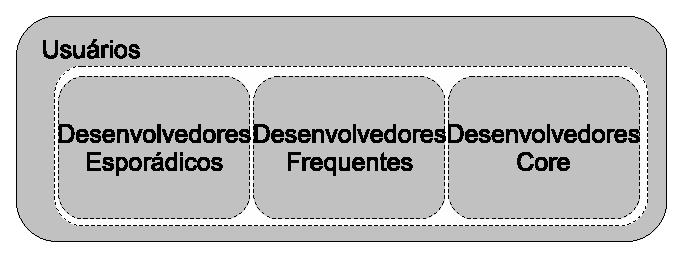
\includegraphics{../../doc/diagramas/equipe.eps}
 % equipe.eps: 1179666x1179666 pixel, 300dpi, 9987.84x9987.84 cm, bb=0 0 482 213
 \caption[Equipe numa comunidade virtual]{Diagrama representando a equipe numa comunidade virtual \cite{introducaoslca}}
 \label{fig:equipe}
\end{figure}

% Trabalhos Relacionados <- Pensar em fazer merge junto com introdução
% Copyright (c) 2008, João Henrique Ferreira de Freitas
% All rights reserved.
% 
% Redistribution and use in source and binary forms, with or without modification,
% are permitted provided that the following conditions are met:
% 
%     * Redistributions of source code must retain the above copyright notice,
%       this list of conditions and the following disclaimer.
%     * Redistributions in binary form must reproduce the above copyright notice,
%       this list of conditions and the following disclaimer in the documentation and/or 
%       other materials provided with the distribution.
%     * Neither the name of the <ORGANIZATION> nor the names of its contributors may
%       be used to endorse or promote products derived from this software without 
%       specific prior written permission.
% 
% THIS SOFTWARE IS PROVIDED BY THE COPYRIGHT HOLDERS AND CONTRIBUTORS "AS IS" AND ANY 
% EXPRESS OR IMPLIED WARRANTIES, INCLUDING, BUT NOT LIMITED TO, THE IMPLIED WARRANTIES
% OF MERCHANTABILITY AND FITNESS FOR A PARTICULAR PURPOSE ARE DISCLAIMED. IN NO EVENT
% SHALL THE COPYRIGHT OWNER OR CONTRIBUTORS BE LIABLE FOR ANY DIRECT, INDIRECT, INCIDENTAL,
% SPECIAL, EXEMPLARY, OR CONSEQUENTIAL DAMAGES (INCLUDING, BUT NOT LIMITED TO, PROCUREMENT
% OF SUBSTITUTE GOODS OR SERVICES; LOSS OF USE, DATA, OR PROFITS; OR BUSINESS INTERRUPTION)
% HOWEVER CAUSED AND ON ANY THEORY OF LIABILITY, WHETHER IN CONTRACT, STRICT LIABILITY,
% OR TORT (INCLUDING NEGLIGENCE OR OTHERWISE) ARISING IN ANY WAY OUT OF THE USE OF THIS
% SOFTWARE, EVEN IF ADVISED OF THE POSSIBILITY OF SUCH DAMAGE.
% 
% $Id$

\section{Referencial Teórico} \label{subsec:referencial}

Há vários estudos relacionados à descoberta de processos de desenvolvimento dentro de comunidades de SL/CA. Muitos investigam as possibilidades de desvendá-los e ao mesmo tempo melhorá-los, reintroduzindo-os no projeto em questão as melhorias evidenciadas como discutido  em \cite{experience}. 

Entretanto outros estudos procuram mapear todo o processo desde a concepção inicial do projeto até a fase de manutenção a fim de fazer comparativos com processos tradicionais da engenharia de software \cite{multimodal} e também estudá-los. 
Em contrapartida, desenvolvedores de SL/CA também são usuários ou administradores dos software que desenvolvem não havendo uma distinção clara entre usuários e desenvolvedores, como observado tradicionalmente no modelo proprietário de desenvolvimento. Visando justamente esta diferença é que se torna importante levantar meios de usuários também atuarem como desenvolvedores e é este o foco do trabalho.

Qualquer desenvolvedor que busque entrar no projeto raramente encontrará informações específicas em qual parte do processo deve atuar. Utilizando uma exploração sistemática, como demonstrado no trabalho de \cite{issue}, na qual busca analisar as informações presentes nos portais oficiais dos projetos através de uma taxonomia \cite{refframework} dos artefatos (discutido com mais profundidate na seção \ref{sec:materiais}), o desenvolvedor aspirante encontrará uma forma de trabalho aparentemente organizada. 

Todavia, muitos autores defendem a idéia que cada projeto de SL/CA não é igual ao outro, possui sua própria engenharia, processos, métodos e formas de comunicação. Felizmente há pontos semelhantes nos quais podem ser utilizados para traçar guias gerais de contribuição.

% TODO: levantar texto que fala sobre "nenhum projeto é igual ao outro"
% \cite{preliminary}
% \cite{acrossweb}
% \cite{multimodal}

% Metodologia Utilizada
% Copyright (c) 2008, João Henrique Ferreira de Freitas
% All rights reserved.
% 
% Redistribution and use in source and binary forms, with or without modification,
% are permitted provided that the following conditions are met:
% 
%     * Redistributions of source code must retain the above copyright notice,
%       this list of conditions and the following disclaimer.
%     * Redistributions in binary form must reproduce the above copyright notice,
%       this list of conditions and the following disclaimer in the documentation and/or 
%       other materials provided with the distribution.
%     * Neither the name of the <ORGANIZATION> nor the names of its contributors may
%       be used to endorse or promote products derived from this software without 
%       specific prior written permission.
% 
% THIS SOFTWARE IS PROVIDED BY THE COPYRIGHT HOLDERS AND CONTRIBUTORS "AS IS" AND ANY 
% EXPRESS OR IMPLIED WARRANTIES, INCLUDING, BUT NOT LIMITED TO, THE IMPLIED WARRANTIES
% OF MERCHANTABILITY AND FITNESS FOR A PARTICULAR PURPOSE ARE DISCLAIMED. IN NO EVENT
% SHALL THE COPYRIGHT OWNER OR CONTRIBUTORS BE LIABLE FOR ANY DIRECT, INDIRECT, INCIDENTAL,
% SPECIAL, EXEMPLARY, OR CONSEQUENTIAL DAMAGES (INCLUDING, BUT NOT LIMITED TO, PROCUREMENT
% OF SUBSTITUTE GOODS OR SERVICES; LOSS OF USE, DATA, OR PROFITS; OR BUSINESS INTERRUPTION)
% HOWEVER CAUSED AND ON ANY THEORY OF LIABILITY, WHETHER IN CONTRACT, STRICT LIABILITY,
% OR TORT (INCLUDING NEGLIGENCE OR OTHERWISE) ARISING IN ANY WAY OUT OF THE USE OF THIS
% SOFTWARE, EVEN IF ADVISED OF THE POSSIBILITY OF SUCH DAMAGE.
% 
% $Id$

\section{Materiais e Métodos} \label{sec:materiais}

%Nesta seção discorreremos sobre como a pesquisa foi elaborada 

Existem várias razões para um usuário colaborar com um projeto de SL/CA. Razões ideológicas, técnicas e necessidades de novas funcionalidades para resolver seus problemas são as mais comuns. Consequentemente, a colaboração ou patch (neste texto os termos colaboração e patch possuem o mesmo sentido\footnote{Patch pode ser definido como sendo uma mudança, conserto ou melhoramento. Incluindo código fonte e documentação. É parte do processo de desenvolvimento SL/CA e muitos projetos possuem guias que descrevem os requisitos para a submissão do patch mas poucos utilizam um processo de revisão e aprovação.\cite{preliminary}}) visam melhoramentos na documentação, suporte a lista de discussão, codificação, manutenção de código e testes. Para todas as contribuições que o usuário pretende fazer, existe um caminho pré suposto no qual se refere aos processos necessários para a colaboração se tornar realmente efetiva no projeto. Um exemplo de uma colaboração não efetiva é a implementação de uma nova funcionalidade que não segue as políticas de codificação e design do projeto em questão, gerando retrabalho ou abandono do patch.

Inicialmente destacamos três softwares no qual gostaríamos de contribuir a fim de codificar determinadas funcionalidades desejadas. Os três softwares são relacionados a infraestrutura de redes, a saber: \textit{Pfsense}\footnote{http://www.pfsense.org}: personalização do sistema operacional FreeBSD para atuar como firewall; \textit{Tikiwiki}\footnote{http://www.tikiwiki.org}: software de gerenciamento de contéudo (CMS); \textit{Bacula}\footnote{http://www.bacula.org}: software de gerenciamento de backup em rede. Mediante ao levantamento inicial realizado, apenas um seria escolhido para a experimentação. A escolha foi feita privilegiando o projeto com maior tempo de vida e estabilidade no ciclo de releases.

% TODO: enquadrar e definir o processo
% - De acordo com o autor, processos são compostos por tarefas e ações atômicas. 
% Cada ação é seguida de entidades: 
% -- agentes participantes da atividade
% -- ferramentas utilizadas pelos agentes para a realização das atividades
% -- recursos que são produzidos e necessários para realizar a atividade
% -- scripts ou métodos contendo a descrição da ação
\subsection{Coleta de Dados} \label{subsection:coletadados}

Cada projeto de SL/CA estabalece métodos próprios de interação, comunicação, liderança e controle. Além das informações dentro da comunidade serem dinâmicas, novos artefatos são inclusos, outros apagados ou desatualizados podendo gerar uma certa frustração na investigação inicial. Felizmente existem diversos frameworks \cite{reference} para tratar a diversidade das informações e torná-las mais padronizadas para a análise de processos num ambiente de SL/CA ou proprietário. Como não era o nosso objetivo descobrir todo o processo de software vinculado ao projeto de SL/CA mas sim uma particularidade comum a todos os projetos de SL/CA, que é a contribuição do usuário no desenvolvimento, não seguimos estritamente um framework para definição de processos.

Na pesquisa realizada, para facilitar a análise do processo colaborativo, além de definir a posição observadora, foi necessário utilizar uma classificação (taxionomia\footnote{Ciência da classificação.}) com componentes que formavam o projeto investigado. Partindo do princípio que toda e qualquer informação de um projeto de SL/CA necessita estar publicamente acessível, iniciamos anotando informações disponíveis publicamente na página oficial do projeto. 

Procuramos traços de informações onde poderíamos encontrar detalhes sobre as relações entre tarefas, ações, atividades, agentes, ferramentas, recursos e padrões utilizados na composição do projeto (figura \ref{fig:mapping}). Esta busca foi denominada de ``entendimento do domínio do'' problema \cite{experience}. Alguns dos principais itens incluíram:

% •  Web pages, including project status reports and task assignments, may be viewed
%   and classified (informally) as object types.
% • Asynchronous communications among project participants posted in threaded
%   email discussion lists, which address process activities indicated by process
%   identifier keywords (e.g., design, release, testing, etc.)
% • Transcripts of synchronous communication via Internet chat (cf. [5]).
%   Software problem/bug and issue reports, which reveal information on software
%   bug reporting and maintenance/repair processes
% • Testing scripts and results, which highlight project-based software testing
%   practices
% • Community newsletters, which highlight project milestone events (e.g., system
%   releases, turnover of core developers in the projects)
% • Web accessible software product source code directories and repositories, which
%   carry timestamps and other identifiers indicating when source code objects were
%   checked in/out, and versioning information.
% • Software system builds (executable binaries) and distribution packages, which are
%   constructed and released on a periodic basis (daily, candidate (alpha, beta), and
%   final release (distribution version)
% • OSS development tools in use in an OSSD project (e.g., concurrent version
%   system (CVS), GNU compiler collection (gcc), bug reporting (bugzilla) (cf. [10])
% • OSS development resources, including other software development artifacts and
%   process fragment descriptions (e.g., How-To guides, lists of frequently asked
%   questions (FAQs), etc.) [26]

\begin{itemize}
 \item Páginas web, relatório de status e atribuições de trabalho;
 \item Comunicação assíncrona entre participantes postadas em listas de discussão via email, no qual endereçavam identificadores de processos (isto é, design, release, testing);
 \item Scripts de teste e resultados, sinalizando processos de testes;
 \item Notícias da comunidade, identificando principais acontecimentos (novas releases ou marcos especiais);
 \item Acessibilidade do repositório de código fonte com identificações, timestamps e versionamentos;
 \item Sistemas de build automáticos;
 \item Ferramentas de desenvolvimento SL/CA utilizadas no projeto (controle de versão, compiladores, gerencia de configuração, bug reporting, framework para testes);
 \item Recursos de desenvolvimento, incluindo outros tipos de artefatos, fragmentos descritivos de processos (isto é, guias (howto), listas de perguntas frequentes (FAQs)).
\end{itemize}

\begin{figure}[h]
 \centering
 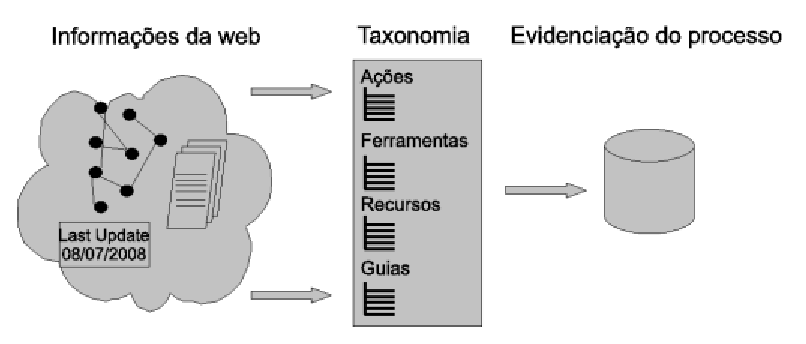
\includegraphics{../../doc/diagramas/maping.eps}
 % maping.eps: -1214733968x146666624 pixel, 300dpi, -10284748.00x1241777.38 cm, bb=0 0 731 292
 \caption[Mapeamento de informações]{Mapeamento de informações, divisão de estruturas e composição de processo \cite{refframework}}
 \label{fig:mapping}
\end{figure}

% - Artefatos comuns: webpages, chats scripts, development resources, process description (howto guides, FAQs)
% 
% - Dimensões dos artefatos: 
% -- Estrutural, how project-related software development artifacts are organizad
% -- Conteudo, tipos de artefatos e informações que eles contém
% -- Pattern de uso, interação do usuário com a comunidade
% -- Pattern de atualização, atualização de conteúdo, criação e remoção

% - Segundo o autor a descoberta do processo específico de um projeto OSSD se inicia com uma exploração no Web space anotando quais informações estão disponíveis e onde podem ser localizadas. Esta exploração nos dá a ideía do que acontece com as ações, agentes, ferramentas e recursos, padrões de utilização a atulização.
% 

Em seguida, classificamos as informações levantadas em três dimensões formadas por:
\begin{itemize}
 \item Estrutural: levantamento de como os artefatos são desenvolvidos e sua organização estrutual;
 \item Conteúdo: levantamentos dos tipos de artefatos e conteúdos;
 \item Padrões de utilização: interação do usuário, desenvolvedores e padrões de atualização com a comunidade.
 \end{itemize}

% The structure of the community Web is evident in two forms. The
% physical form consists of the directory structure of the files of
% which the site is composed. But, it is also apparent on a logical
% level, in terms of the site layout, as might be given by a site map
% or menu. These may or may not be equivalent. Nevertheless,
% each layer in the hierarchy provides a clue to the types of agents,
% resources, tools, and processes of the community. Structure
% hierarchy names may be mapped to instances of tools, agents,
% resources, and activities found in the open source software
% development meta-model taxonomy, thus fulfilling the first role
% of the reference framework.
A organização estrutural da comunidade geralmente é evidente na hierarquia organizacional adotado pelo web site do projeto em função de seu layout e diretórios de acesso. Diretórios com grande número de arquivos e arquivos grandes podem indicar intensa atividade como observado em listas de email e fórums, repositório de código fonte, notícias da comunidades, repositórios de \textit{issue}, seções de release e \textit{changelogs}, entre outras. A presença destes itens indicam um processo de desenvolvimento.

% Additionally, directories with a high
% amount of content, both due to file numbers and file size may
% indicate a focus on activity in that area. Claims such as these may
% then be reinforced or refuted based on additional information
% gathered during discovery. Common to most open source
% communities are mailing lists and discussion forums, source
% repositories, community newsletters, issue repositories, and
% binary release sections, among others. The mere presence of
% these suggests certain activities in the development process.

As relações começam a se tornar mais evidentes quando investigamos o conteúdo do repositório de código fonte e relacionamos com um bugtracker\footnote{É um sistema desenvolvido para ajudar no gerenciamento de bugs a fim de melhorar a qualidade do sistema a ser desenvolvido. Geralmente um bug tracker é uma porção menor de um issue tracker, \url{http://en.wikipedia.org/wiki/Bugtracker}} ou issuetracker\footnote{Issue é uma unidade de trabalho com o objetivo de melhoramento. Pode ser um bug, melhoramento, tarefa, documentação, entre outras. Tradicionalmente issue pode ser traduzido como \textit{problema}, \url{http://en.wikipedia.org/wiki/Issue_tracking_system}}. Esta relação diz como as mudanças no código fonte são realizadas e se há algum processo de teste implantado. Em algumas comunidades o banco de dados de issue também é utilizado para requisitar novas features, enquanto que em outras geralmente encontramos em forums ou listas de discussão. Entretanto iremos encontrar a maioria dos dados relacionados nas páginas web, em mensagens de email, guias gerais e tudo que possa compor um quadro de informações autocontido.


% These also signal what types of data may be contained therein. If
% we just look at source repositories, we can obtain a process
% specification of a limited set of activities- those that involve
% changes to the code, just as issue and bug databases tell us that
% some testing is done on which the issue reports are based. In
% some communities, issue reports are also used to file feature
% requests. Such information may also be found within discussion
% forums or email lists.
% 


% The bulk of the process data is found within the content of Web
% artifacts. Much of the mapping consists of text matching between
% strings in artifacts such as web pages, and email messages and
% process related keywords as was demonstrated for structure-based
% data. In the case of web content, we are also looking for items
% like date stamps on email messages to place the associated events
% in time, document authors, and message recipients. In some
% cases, it is possible to uncover “how-to” guides or partial process
% prescriptions. Like other content, these may not accurately reflect
% the process as it is currently enacted, if they ever did. Therefore,
% each datum must be verified by others.

Padrões de uso são indicadores das principais áreas do espaço web mais ativas, reforçando a validação dos dados encontrados e quais atividades do processo estão ocorrendo em determinado tempo. Podem ser evidenciadas via contadores de acesso e estatísticas de última atualização.

% Usage patterns, like content size, are indicators of which areas of
% the Web space are most active, which reinforces the validity of
% the data found therein and also what activities in the process may
% be occurring at a given time. Web access logs, if available,
% provide a rich source of data. Page hit counters and last update
% statistics are also useful for this purpose. 

% OSSD artifacts vary along these three dimensions over time, and
% this variance is the source of process events. To effectively
% discover processes, our reference framework must be able to
% relate artifacts in the community Web space with process actions,
% tools, resources, and roles.

Artefatos de desenvolvimento SL/CA variam dentro das três dimensões (estrutural, conteúdo, padrões de utilização) durante todo o tempo. A análise se torna mais efetiva quanto mais minuciosa for a classificação executada e o cruzamento dos dados com a engenharia de software tradicional.

% 
% - Em uma organização é possível determinar algumas coisas olhando para um gráfico organizacional e coisas do tipo. Já em um projeto open-source não há este tipo de artefato.
% 
% - O processo de engenharia de requisitos é diferente do tradicional (elicitação, especificação, análise, modelagem, comunicação e gerenciamento)
% 
% 
% 

% - Casos de uso podem ser utilizados para demonstrar as interrealções das ações, utilização de ferramentas e atores. Os casos de uso podem ser integrados para produzirem um conteúdo de hypermedia relacionando todas as atividades do processo.




% Exposição de experiências
% Copyright (c) 2008, João Henrique Ferreira de Freitas
% All rights reserved.
% 
% Redistribution and use in source and binary forms, with or without modification,
% are permitted provided that the following conditions are met:
% 
%     * Redistributions of source code must retain the above copyright notice,
%       this list of conditions and the following disclaimer.
%     * Redistributions in binary form must reproduce the above copyright notice,
%       this list of conditions and the following disclaimer in the documentation and/or 
%       other materials provided with the distribution.
%     * Neither the name of the <ORGANIZATION> nor the names of its contributors may
%       be used to endorse or promote products derived from this software without 
%       specific prior written permission.
% 
% THIS SOFTWARE IS PROVIDED BY THE COPYRIGHT HOLDERS AND CONTRIBUTORS "AS IS" AND ANY 
% EXPRESS OR IMPLIED WARRANTIES, INCLUDING, BUT NOT LIMITED TO, THE IMPLIED WARRANTIES
% OF MERCHANTABILITY AND FITNESS FOR A PARTICULAR PURPOSE ARE DISCLAIMED. IN NO EVENT
% SHALL THE COPYRIGHT OWNER OR CONTRIBUTORS BE LIABLE FOR ANY DIRECT, INDIRECT, INCIDENTAL,
% SPECIAL, EXEMPLARY, OR CONSEQUENTIAL DAMAGES (INCLUDING, BUT NOT LIMITED TO, PROCUREMENT
% OF SUBSTITUTE GOODS OR SERVICES; LOSS OF USE, DATA, OR PROFITS; OR BUSINESS INTERRUPTION)
% HOWEVER CAUSED AND ON ANY THEORY OF LIABILITY, WHETHER IN CONTRACT, STRICT LIABILITY,
% OR TORT (INCLUDING NEGLIGENCE OR OTHERWISE) ARISING IN ANY WAY OUT OF THE USE OF THIS
% SOFTWARE, EVEN IF ADVISED OF THE POSSIBILITY OF SUCH DAMAGE.
% 
% $Id$

\section{Resultados e Discussão} \label{sec:resultados} \label{subsec:sobre}

A taxionomia (vide anexo \ref{sec:anexob}) realizada inicialmente foi deixada em segundo plano, na forma de consulta sempre que dúvidas relacionado aos artefatos do projeto surgiram. Uma espécie de guia de consulta rápida onde foi possível determinar as próximas ações para determinada atividade como por exemplo testes de regresão, submissão de patch, padrões de codificação e design.

Antes de iniciarmos a discussão da experiência, é necessário posicionar o leitor nos recursos desejados e implementados no projeto de SL/CA escolhido anteriormente. Em resumo a funcionalidade desejada (vide anexo \ref{sec:anexoa}) era o suporte a uma camada de abstração no software de gerenciamento de backups de rede \textit{Bacula}. Antes do nosso patch (denomidado \patch ou simplesmente \patchshort), o software Bacula contava apenas com o suporte a SGBDs livres (Mysql, Postgresql e SQLite) nos quais eram implementados nativamente, via APIs (Application Programming Interface ou Interface de Programação de Aplicativos) padrões para acesso aos SGBDs específico, no código do Bacula. 

A implementação de uma camada de abstração possibilitou a integração com outros SGBDs livres ou proprietários (vide anexo \ref{sec:anexod}) sem mudanças no código do Bacula, ou com mudanças mínimas.\footnote{Na realidade, como há diversos dialetos para a linguagem SQL implementada nos SGBDs, torna-se necessário revisar as consultas utilizadas pelo Bacula antes do mesmo suportar oficialmente outro SGBD.} Além de possibilitar um único ponto de manutenção para o código referente ao interfaceamento com SGBDs. Nas seções seguintes, apresentamos os detalhes da implementação e também o modelo de desenvolvimento utilizado.

\subsection{Implementação do patch} \label{sec:anexoe}

O software Bacula é um conjunto de softwares (vide figura \ref{fig:arqbacula}) no qual permitem gerenciar \textit{backups}, \textit{restores} e verificações através da rede de diversos tipos de computadores. Bacula é relativamente fácil de usar e eficiente, oferece muitos meios de armazenar os dados e recursos para gerenciá-los, procurá-los e recuperá-los. A maioria do código fonte está licenciada sob a licença GPL versão 2 e com direitos passados para a Free Software Foundation Europa.

Como podemos notar na figura \ref{fig:arqbacula} o software Bacula possui um conjunto de programas nos quais podem ser instalados e executados em diferentes máquinas dentro de uma rede.
Os principais componentes são:
\begin{itemize}
\item Servidor de Backup, denominado de \textit{bacula-dir}, com as funções de orquestrar toda a solução;
\item Servidor de Armazenamento, denominado de \textit{bacula-sd}, responsável por armazenar todos os arquivos enviados pelos bacula-fd;
\item Servidor de Arquivos, denomindado de \textit{bacula-fd}, responsável por enviar para o bacula-sd os arquivos necessários para serem armazenados provenientes dos computadores de uma rede;
\item Estações de Administração, denomindas de \textit{console}, são utilizadas para controlar via linha de comando ou interface gráfica as operações e tarefas do Bacula;
\item Servidor de Banco de Dados, denominado \textit{catalog database} ou banco de dados, armazena os meta-dados (características de cada arquivo).
\end{itemize}

\begin{figure}[h]
 \centering
 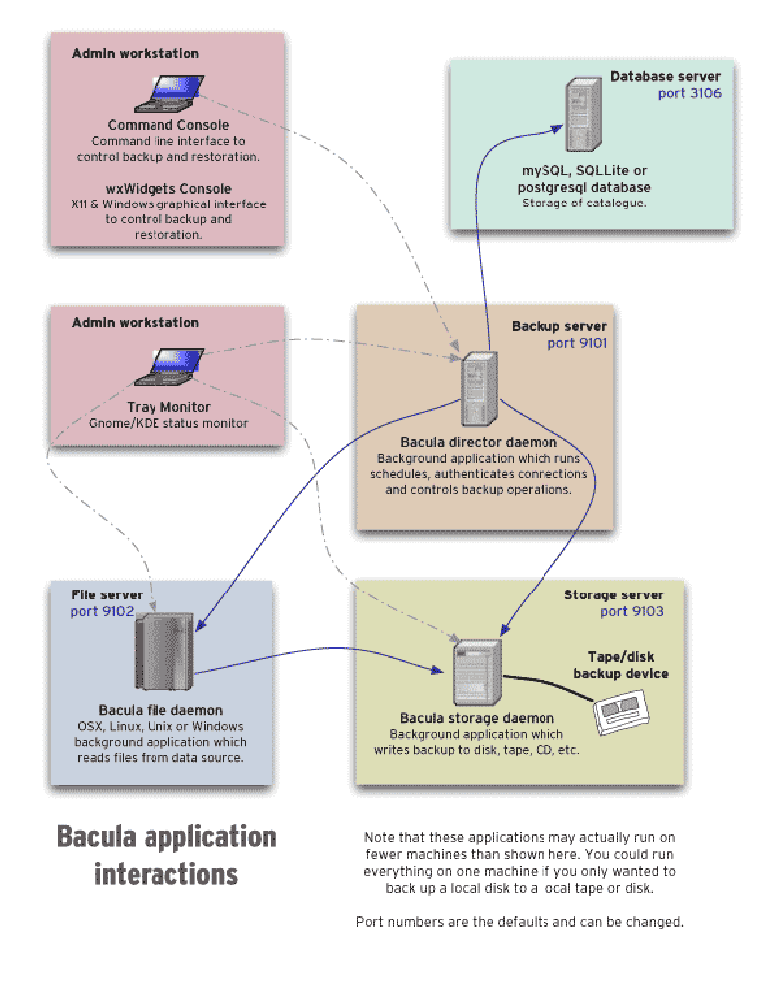
\includegraphics[scale=0.8]{../../doc/figuras/bacula-applications.eps}
 % bacula-applications.png: 1179666x1179666 pixel, 0dpi, infxinf cm, bb=
 \caption[Arquitetura geral do Bacula]{Arquitetura geral do sistema \\ \url{http://www.bacula.org/en/dev-manual/What_is_Bacula.html}}
 \label{fig:arqbacula}
\end{figure}

Durante a implementação do patch \patchshort, concentramos apenas nos componentes bacula-dir e catalog database. Não tivemos a necessidade de interferir nos outros componentes do sistema pois tratavam operações nas quais não nos interessavam no momento.

Para ajudar no entendimento, a figura \ref{fig:comparativo} oferece uma visão geral  antes e depois da implementação do patch. 

Na figura \ref{fig:unico} notamos a utilização de um único banco de dados por binário, ou seja, a escolha de qual banco de dados utilizado é definida durante a compilação do código fonte do Bacula, no qual eram definidos os códigos necessários para construir o driver de acesso nativo via API própria de cada banco de dados. A camada sql\_\*.c utiliza as funções definidas em [banco de dados].c,  onde [banco de dados] pode ser apenas um dentre: mysql, postgresql, sqlite. Desta forma, uma vez compilado, o usuário apenas utilizaria o banco de dados escolhido. 
Um outro ponto é o suporte aos bancos de dados limitados, ou seja, apenas para os SGBDs codificados no Bacula.

Já na figura \ref{fig:dbi} observamos um novo cenário no qual uma camada de abstração (via bibliotema libdbi) e um driver (dbi.c) para fazer a interface entre a camada sql\_\*.c e a libdbi foi implementado. Basicamente para garantir dois pontos: 
\begin{itemize}
\item O primeiro é a independência do banco de dados a ser utilizado pelo Bacula. 
\item O segundo ponto é a possibilidade de utilizar vários tipos de SGBDs para armazenar meta-dados de arquivos.                                                                   \end{itemize}
Um exemplo do segundo ponto abordado é a possibilidade de realizar backups entre bancos de dados ou até mesmo a transferência de um catálogo de um banco de dados para outro completamente distinto em caso de problemas ou manutenções.

\begin{figure*}[h]
 \centerline{
  \subfigure[Único banco de dados por binário]{
  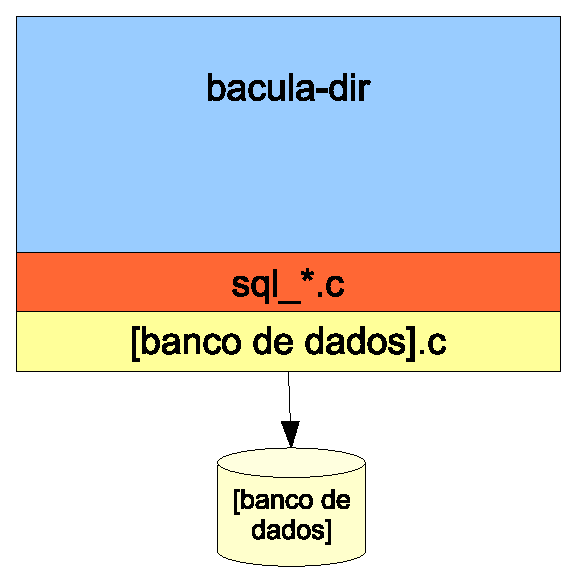
\includegraphics[width=5cm]{../../doc/diagramas/bacula-dir-sgbd.eps}
  \label{fig:unico}
  }
  \hfil
  \subfigure[Vários tipos de banco de dados por binário]{
  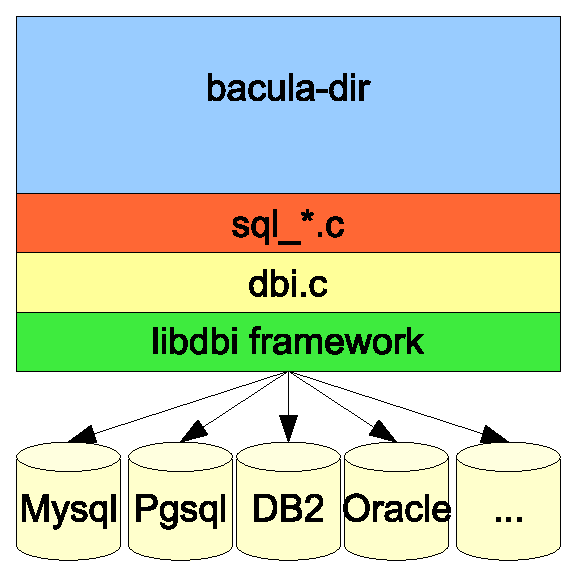
\includegraphics[width=5cm]{../../doc/diagramas/bacula-dir-dbi.eps}
  \label{fig:dbi}
  }
 } 
 \label{fig:comparativo}
 \caption[Comparativo de implementação]{Comparativo da implementação realizada \subref{fig:unico} e \subref{fig:dbi}}
\end{figure*}

\subsubsection{Limitações}

A principal limitação encontrada é referente a existência de diversos tipos de SGBDs utilizando diferentes dialetos e recursos da linguagem SQL. Não é possível prever todos os casos. Há consultas que funcionam em todos os SGBDs e outras que são específicas e devem ser tratadas a parte. 

A biblioteca libdbi oferece uma abstração para os diferentes tipos de APIs de cada fabricante de SGBDs mas a mesma não oferece nenhum suporte aos diferentes tipos de SQL utilizados por eles.

Sendo assim o Bacula deve ser preparado para suportar os diferentes dialetos SQL, ou seja, para cada banco de dados temos um conjunto de SQL que devem ser adptadas e suportadas para que o SGBD seja efetivamente suportado. Isso se torna uma limitação pois necessita de uma intervenção no código para o correto funcionamento.

\subsubsection{Implementação}

As tarefas de criação do ambiente necessário para a implementação e definição de quais arquivos seriam necessários criar ou alterar não foram complicadas. Notamos um software bem modularizado e dividido para facilitar a manutenção e adiçaõ de novos recursos. A seguir apresentamos uma macro lista dos itens no qual foram necessário trabalhar:

\begin{itemize}
\item Alteração no arquivo \url{src/cats/cats.h}: 
 \subitem inclusão da regra de compilação condicional HAVE\_DBI para o compilador reconhecer o código para o driver DBI
 \subitem adaptado a estrutura de dados B\_DB, responsável pelo gerenciamento de todos os itentes relacionados a banco de dados, dentro do Bacula, bem como as definições de várias funções para a API da libdbi
\item Alteração dos arquivos \url{src/cats/sql*.c}: incluindo a regra de compilação condicional HAVE\_DBI
\item Criado o arquivo \url{src/cats/dbi.c} baseado no código \url{src/cats/postgresql.c}
 \subitem tranformado e convertigo as funções presentes no arquivo src/cats/dbi.c de um código com APIs referentes ao SGBD postgresql para APIs da  biblioteca DBI. Evidente que muitas funções presentes no SGBD postgresql não seguiam a mesma lógica utilizada na biblioteca DBI. Sendo necessário estudar as documentações e códigos de ambas para entender o funcionamento e decidir se a API da biblioteca DBI atendia ou não a forma na qual o Bacula estava projetado para interagir com um SGBD. 
\item Alterado o arquivo \url{src/dird/dird_conf.h} e \url{src/dird/dird_conf.c}
 \subitem adicionado a opção de configuração dbdriver no qual informava ao Bacula qual driver e banco de dados será utilizado.
\item Alterado os arquivos \url{src/autoconf/config.h.in} e \url{src/autoconf/bacula-macros/db.m4} referentes a geração do script de autoconfiguração para compilação, baseados nas disponibilidades dos requisitos da plataforma.
\item Adaptação de todos os testes de regressão para incluir as opções de configuração para o driver DBI
\end{itemize}

\subsubsection{Timeline do desenvolvimento}
\begin{table}[htbp]
\begin{tabular}{|l|c|c|c|c|}
\hline
 & \textbf{Data} & \textbf{Submissões} & \textbf{Data Integração} & \textbf{Revision} \\ \hline
\multicolumn{ 1}{|c|}{\textbf{Exploração Arquitetural}} & 2007-12-07 &  &  &  \\ \cline{ 2- 5}
\multicolumn{ 1}{|l|}{} & 2008-01-11 &  &  &  \\ \hline
\multicolumn{ 1}{|c|}{\textbf{Desenvolvimento}} & 2008-01-18 &  &  &  \\ \cline{ 2- 5}
\multicolumn{ 1}{|l|}{} &  & 2008-02-01 & 2008-02-02 & 6358 \\ \cline{ 2- 5}
\multicolumn{ 1}{|l|}{} &  & 2008-02-12 & 2008-02-13 & 6413 \\ \cline{ 2- 5}
\multicolumn{ 1}{|l|}{} &  & 2008-02-19 & 2008-02-22 & 6464 \\ \cline{ 2- 5}
\multicolumn{ 1}{|l|}{} &  & 2008-02-21 & 2008-02-27 & 6498 \\ \cline{ 2- 5}
\multicolumn{ 1}{|l|}{} &  & 2008-02-25 & 2008-04-15 & 6825 \\ \cline{ 2- 5}
\multicolumn{ 1}{|l|}{} &  & 2008-03-17 & 2008-04-15 & 6826 \\ \cline{ 2- 5}
\multicolumn{ 1}{|l|}{} &  & 2008-04-09 & 2008-04-09 & 6817 \\ \cline{ 2- 5}
\multicolumn{ 1}{|l|}{} &  & 2008-04-14 & 2008-04-15 & 6818 \\ \cline{ 2- 5}
\multicolumn{ 1}{|l|}{} &  & 2008-04-27 & 2008-04-27 & 6874 \\ \cline{ 2- 5}
\multicolumn{ 1}{|l|}{} & 2008-05-02 &  &  &  \\ \hline
 &  &  &  &  \\ \hline
 & \textbf{Orçadas} & \textbf{Trabalhadas} &  &  \\ \hline
\textbf{Exploração Arquitetural:} & 64h & 59.89h &  &  \\ \hline
\textbf{Desenvolvimento:} & 168h & 118h &  &  \\ \hline
\end{tabular}
\caption{Timeline}
\label{Timeline}
\end{table}

\subsection{Modelo de desenvolvimento utilizado durante o experimento} 

Durante toda a experiência, como não tinhamos muito bem definido os requisitos necessários para a implementação. E tão pouco um conhecimento suficiente grande do código em que iriamos modificar, foi necessário utilizar um modelo de desenvolvimento no qual fosse permitido definir um mínimo de objetivos e logo iniciar o ciclo de desenvolvimento, após uma fase de \textit{Exploração Arquitetural}. 

Atrelando ao fato de que o projeto Bacula estabelece frameworks de testes e recomendações explícitas para a utilização sempre após qualquer alteração no código fonte, e tendo em consideração que uma das premissas para a utilização do modelo em vista era uma forma de validação da implementação rapidamente para que nada fosse alterado de forma a quebrar as outras funcionalidade existentes. Achamos pertinente utilizar o modelo de \textit{Programação ou Desenvolvimento Exploratório} (vide figura \ref{fig:exploratoria}). 

Em \cite[página 31]{engenharia1} define como sendo: \textit{``O modelo de programação ou desenvolvimento exploratório visa a construção da primeira versão do sistema o mais rápido possível. Sistemas desenvolvidos assim caracterizam-se por não terem o escopo claramente definido... Após o desenvolvimento de cada uma das versões do sistema, ele é mostrado aos usuários para comentários. Modificações sucessivas são feitas no sistema até que o mesmo seja considerado adequado''}.

\begin{figure}[h]
 \centering
 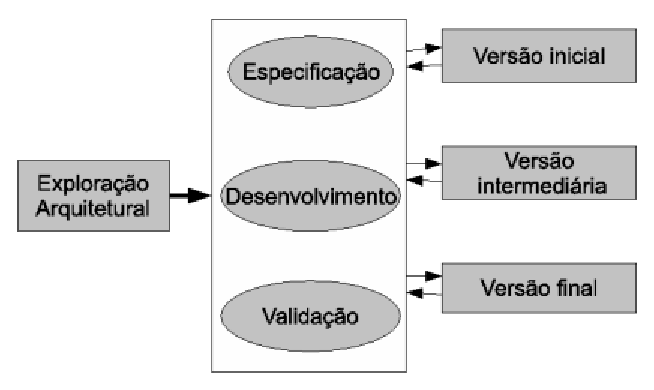
\includegraphics{../../doc/diagramas/programacao_exploratoria.eps}
 % programacao_exploratoria.eps: 1179666x1179666 pixel, 300dpi, 9987.84x9987.84 cm, bb=14 14 312 185
 \caption[Programação exploratória]{Modelo de programação exploratória \cite{engenharia1}}
 \label{fig:exploratoria}
\end{figure}

Acreditamos que não havendo um framework de testes, no qual realizamos diversos testes de regressão no projeto, não seriamos capazes de implementar as modificações propostas. Devido as chances de quebrar toda a consistência dos dados do software. Do ponto de vista do desenvolvedor, testes automáticos encorajam o desenvolvimento e aumentam o processo de \textit{refactoring}\footnote{Processo de constantes melhorias no design e código do software}\cite[página 203]{producing}.

% Exploratory programming is an important part of the software engineering cycle: when a domain is not very well understood or open-ended, or it's not clear what algorithms and data structures might be needed for an implementation, it's useful to be able to interactively develop and debug a program without having to go through the usual constraints of the edit-compile-run-debug cycle.
%  
% "Automated testing"
%
% TODO: Elaborar um texto de introdução

\subsubsection{Exploração Arquitetural e Escopo}\label{subsec:arquiterual}\label{subsec:experiencia}

%\textit{Como planejar os melhoramento e qual a melhor forma de planeja-los?}\\
Após a elaboração da classificação, de acordo com o anexo \ref{sec:anexob}, iniciamos os experimentos elaborando os requisitos necessários (vide anexo \ref{sec:anexoa:baculalibdbi}) para as melhorias objetivadas para o projeto.

Basicamente tentamos responder os seguintes questionamentos: \textit{O que?}, realmente precisamos desta funcionalidade; \textit{Porque?}, quais os fundamentos técnicos e benefícios para o projeto implementando esta funcionalidade; \textit{Como?}, quais os artefatos necessários e como implementá-los (vide anexo \ref{sec:anexoa:featurereq}). Evidente que para a última questão um conhecimento maior sobre o software em si foi necessário antes de aventurarmos em sugestionar mudanças para a comunidade do projeto. Entretanto a dificuldade relacionada em argumentar como a nova funcionalidade desenvolvida se encaixou no software foi minimizada via uma \textit{Exploração Arquitetural}, demonstrada adiante.

A melhor definição de Exploração Arquitetural (EA) é encontrada dentro do modelo de desenvolvimento XP no qual também possui uma fase exploratória e pode ser definido, segundo \cite[página 36]{procdesenv}: \textit{``A fase de exploração é anterior à construção do sistema. Nela, investigações de possíveis soluções são feitas e verifica-se a viabilidade de tais soluções... Os clientes são consultados e trazidos para dentro da equipe... Os programadores são responsáveis por fazer experimentos com a possível tecnologia e infra-estrutura a ser escolhida...''}. No contexto do trabalho, entendemos que ``clientes'' são os desenvolvedores do núcleo do projeto com uma visão mais crítica das modificações propostas e ``programadores'' são os contribuidores do patch. Asssim a visão do XP se encaixa perfeitamente para a experiência.

% Explicar melhor oque foi feito com a Exp. Arq. fazendo ref. para os emails e testes realizados anteritormente
% É a hora de usar a taxocomia em busca de informaçòes de como fazer. Relatar a procura no svn, emails antigos, guias de referencias, comunicação com outros projeto

Enfim, a Exploração Arquitetural possibilitou as atividades abaixo relacionadas e um conhecimento maior sobre o projeto de SL/CA e sua engenharia. 
\begin{description}
\item [Testar as possibilidades] ponto em que o desenvolver percebe o mal funcionamento, necessidade de manutenção ou implementação de uma nova fucionalidade.
\item [Documentar as necessidades] para levantamento e descrição dos requisitos, escopo inicial e analise de como fazer a modificação (vide anexo \ref{sec:anexoa}).
\item [Levantar feedback dos desenvolvedores] abrindo discuções formalmente, via lista de discussão ou email privado com os desenvolvedores. É importante nesta fase a argumentação técnica das modificações a serem realizadas e evidenciar os benefícios para o projeto. Muitas vezes é a partir deste ponto que a modificação pode ou não dar certo (vide anexo \ref{sec:anexod})
\item [Iniciar experimentações]: implementação dos requitisos e testes. Neste ponto os testes são fundamentais pois as novas funções ou modificações não devem quebrar o código já existente.
\item [Analisar possibilidades]: ponto em que o desenvolvedor envia os patches para aprovação pelos desenvolvedores oficiais do projeto e recebe os maiores feedbacks sobre seu trabalho.   \end{description}

É importante ressaltar que as fases \textit{Documentar as necessidades} e \textit{Levantar feedback dos desenvolvedores}, na experiência, ocorreram quase que concomitantemente devido a necessidade de saber a viabilidade da implementação para não precisar abortar os trabalhos ou se tornar inviável devido alguma barreira (vide discussões no anexo \ref{sec:anexod} para maiores detalhes).

Mesmo que o contribuidor não conheça a fundo o projeto objetivado, através da EA ele poderá se sentir confortável, ou seja, saber como e onde os artefatos do projeto se encaixam e manter um diálogo saudável com a comunidade de desenvolvedores, para realizar as implementações necessárias.
% Caminho 1: Oque deseja implementar pode estar na árvore de código do projeto. Você pode consultar o repositório em busca de logs de alterações. Geralmente as alterações são atômicas para determinados requisitos, ou seja, aparecem por inteiro provenientes de um desenvolvedor.

% Exploração arquitetural e técnica
%     Levantamento de informações relacionadas ao projeto em questão;% 
%     Necessidade de conhecer o projeto e sua engenharia pois cada um possue suas particularidades.
% 
%     Alguns detalhes importantes:
% 
%     * políticas de release
%     * documentação
%     * padrões de desenvolvimento
% 
%  
% 
%     Modelo sugerido
% 
%  
% 
%                |-----------\  |--------\    |--------------\     |--------------\ 
%        exploração          \           \                   \                    \ 
%                            analise     \                   \                    \ 
%                                       projeto              \                    \ 
%                                                          desenvolvimento        \
%                                                                               testes
% 
%                |------------------------------------||---------------------------------------|
% 
%                       foco do trabalho                            anexo do trabalho
% 
%  
% 

\subsection{Ciclo de desenvolvimento}

Após o período necessário para entendimento do projeto Bacula, iniciamos as primeiras experiências na implementação do patch. Já havíamos traçado os planos em discussões com desenvolvedores de quais arquivos seriam necessários trabalhar e os pontos de maior cautela. Para maiores detalhes relacionado a implementação do patch (código e arquitetura) vide anexo \ref{sec:anexoe}.

\subsubsection{Padrões de projetos identificados}

Basicamente o Bacula é um software multiplataforma escrito em C/C++ com um design e codificação muito claros, bem estruturado e modular. O entendimento do código fonte não foi um problema por dois motivos: 
\begin{enumerate}
\item O projeto possue um documento de guias gerais de implementação (vide anexo \ref{sec:anexob}) no qual foi fundamental para o entendimento de diversos pontos relacionado aos padrões de desenvolvimento e arquitetura;
\item Por se tratar de uma codificação modular tinhamos a oportunidade de ler o código mais claramente e buscar rapidamente a função ou parte do código que tinhamos a necessidade de entender.
\end{enumerate}
Durante o desenvolvimento utilizamos a biblioteca (ou framework) libdbi\footnote{\url{http://libdbi.sourceforge.net/}} (vide anexo \ref{sec:anexog}), no qual permitiu o acesso aos diversos SGBDs. O ponto de maior dificuldade foram as experiências necessárias para saber como a biblioteca libdbi funcionava e como integrá-la ao projeto da melhor forma possível, ou seja, utilizando as estruturas de dados e técnicas semelhante aos \textit{drivers} já implementados, no Bacula, para acesso aos bancos de dados nativamente. Assim, grande parte do tempo foi dedicado a esta integração. 

\subsubsection{Ferramentas utilizadas}

Diversas ferramentas deram suporte às atividades ao longo do projeto e podem ser divididas em três grupos: 
\begin{itemize}
 \item Gerênciais: utilização da ferramenta \textit{dotProject}\footnote{\url{http://www.dotproject.net/}} no qual funcionou como gerenciador do projeto e controle de horas gastas;
 \item Técnicas: \textit{subversion}, para gerenciamento do código fonte; \textit{eclipse} com plugin para C/C++, utilizado como IDE e navegação no código fonte; \textit{ddd}\footnote{\url{http://www.gnu.org/software/ddd/}}, para debug do código; \textit{valgrind}\footnote{\url{http://www.valgrind.org}}, para profiling de memória e deteção de vazamentos de memória;
 \item Operacionais: bancos de dados Postgresql e Mysql; sistema operacional Ubuntu Linux 7.10.
\end{itemize}

\subsubsection{Dia a dia de trabalho}
O período de desenvolvimento pôde ser dividido nas atividades de implementação, testes, análise, discussão de problemas e submissão do patch. A figura \ref{fig:resolucao_problemas} ilustra o relacionamento entre cada atividade. 
\begin{figure}[h]
 \centering
 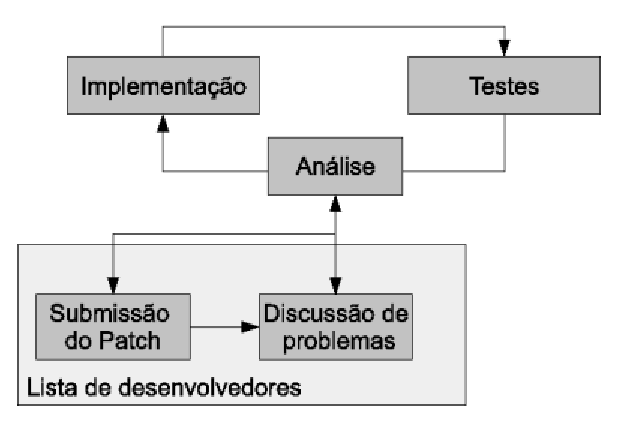
\includegraphics{../../doc/diagramas/resolucao_problemas.eps}
 % resolucao_problemas.eps: 1179666x1179666 pixel, 300dpi, 9987.84x9987.84 cm, bb=0 0 431 287
 \caption[Fase de desenvolvimento]{Fase de desenvolvimento utilizada na experimentação}
 \label{fig:resolucao_problemas}
\end{figure}

Podemos identificar que as atividades de implementação, testes e análise ocorreram de forma circular, ou seja, a cada implementação foi seguida por testes e anaĺise dos resultados. Havendo problemas ou dúvidas; eram reportadas via lista de discussão, voltando para o ciclo de implementação e verificando se os problemas reportados na lista de desenvolvimento foram sanados. Todo o ciclo se repetiu até que a implementação do patch \patchshort fosse validada, testada e integrada no repositório do projeto Bacula.

Trabalhando desta maneira, conseguimos fazer com que os desenvolvedores sugestionassem e mudassem o design caso houvesse necessidade (vide anexo \ref{sec:anexod:problemas} para mais detalhes). 

Abaixo descrevemos as atividades:

\begin{description}
\item[Implementação]: tarefas relacionadas à codificação, experimentações e sincronização com o ramo principal de desenvolvimento do projeto. As sincronizações são necessárias sempre antes de iniciar os trabalhos para verificar se nada mudou em outras partes do código fonte.
\item[Testes]: a cada codificação os testes de regressão (ou quaisquer outros) devem ser executados.
\item[Análise]: basicamente é a verificação dos testes e problemas encontrados na implementação. Caso ocorra dificuldade tais como: mudanças extremas em várias partes do código, dúvidas referentes ao design do software, mudanças de conceitos, é necessário entrar em contato com os desenvolvedores e expor os problemas encontrados.
\item[Discussão]: as necessidades especiais e problemas devem ser expostas afim de coletar feedback do trabalho e também sanar os problemas, como por exemplo: mudança de design, alteração de nomes, modificação de técnicas.
\item[Submissão]: durante a fase de análise, caso identifiquemos que o patch esta suficientemente maduro para ser submetido ou queremos demonstrar o status do trabalho, devemos submete-lo na lista de desenvolvimento para algum outro desenvolvedor possa testar, revisar e possivelmente integrar na árvore principal de código fonte do projeto.
\end{description}

\subsubsection{Submissão do patch}

Após o período de desenvolvimento, no qual não foi finalizado até a execução satisfatória de todos os testes de regressão do projeto Bacula, o patch \patchshort foi submetido na lista de desenvolvimento. 

Mediante as regras de licenciamento do projeto, de acordo com anexo \ref{sec:anexoc}, o patch só pôde ser aceito e integrado no repositório do projeto após o envio por carta convencional contendo a doação formalmente do código escrito para o projeto. Segundo os desenvolvedores esta é uma medida de proteção para evitar problemas legais referentes a patentes de software. 
Após o recebimento\footnote{A carta foi destinada a \textit{Free Software Foundation Europa} (\url{http://www.fsfeurope.org/}) mais especificadamente para o projeto conhecido como \textit{Freedom Task Force} (\url{http://www.fsfeurope.org/projects/ftf/about.pt.html})} da carta, o código pôde ser integrado.

Identificamos três tipos de submissões ao longo do processo de desenvolvimentos:

\begin{description}
\item[Submissão temporal] ocorreu quando houveram algumas necessidades: mostrar o status do trabalho para os desenvolvedores do núcleo, integrar código no repositório principal do projeto para testes, levantar feedback técnico a respeito da implementação (vide anexo \ref{sec:anexod:submissaotemporal}).
\item[Submissão de finalização] após a implementação, execução de todos os testes de regressão e limpeza no código fonte. Foi feita a submissão final para integração no repositório (vide anexo \ref{sec:anexod:submissaofinal}).
\item[Submissão de manutenção] consequentemente o patch \patchshort se tornou oficial e entrou num período de manutenção. Neste período podem ocorrer manutenção e melhoramentos no código, gerando submissões de manutenção (vide anexo \ref{sec:anexod:submissaomanutencao}).
\end{description}

É importante notar que não foi dado permissões de integração do código diretamente no repositório do projeto, mesmo após o envio da referida carta. Acreditamos que a razão foi a codificação de uma melhoria específica e ser a primeira vez que temos contato com o projeto Bacula.

\subsection{Exposição dos resultados}

No contexto da experiência realizada, após cinco meses de pesquisas, interações com  comunidades e desenvoldores para a resolução de todos os obstáculos técnicos encontrados, conseguimos estabilizar o patch \patchshort para integrá-lo em uma versão estável do projeto Bacula. Completando assim nossos objetivos de contribuir e capturar o processo de implementação de um patch dentro da comunidade de SL/CA. 

Na seção \ref{sec:objetivos} colocamos algumas questões inicialmente levantadas antes de iniciarmos os experimentos acima discutidos. Com o auxílio dos experimentos realizados, responderemos cada pergunta de maneira a expor as recomendações, evidenciadas nesta experiência, para futuros contribuidores em projetos de SL/CA:

\textit{Quais os caminhos e possibilidades para usuários colaborarem?} Dentre os itens comumente citados para usuários colaborarem, tais como implementação de código, testes, documentações, tradução, entre outros. Projetos de SL/CA são carentes em contribuidores que possam ajudar a definir melhores processos de desenvolvimento dentro da engenharia de software tradicional. Definir melhor não significa que os processos não existam mas sim corrigir a forma nas quais as atividades e processos ocorrem. Por exemplo: sentimos dificuldades em descobrir e verificar o status das tarefas nas quais os desenvolvedores do núcleo estavam realizando.

\textit{Como colaborar efetivamente?} A efetividade em projetos de SL/CA está ligado ao nível de conhecimento que o contribuidor possui. Por exemplo: caso ele tenha conhecimentos avançados em uma determinada linguagem de programação, é mais fácil para ele implementar códigos mais ousados, eficientes e seguros. Felizmente não é necessário possuir grandes conhecimentos para iniciar as atividades de contribuição. Numa vertente não técnica: comunicar-se e descobrir o processo utilizado pela comunidade de SL/CA e na vertente técnica analisar e entender o código fonte em busca de reaproveitamento, modularidade e averiguando como implementar o necessário sem quebrar a consistência e padronização do projeto.

% Conlusão 1: O desenvolvedor que se aventura em projetos SL/CA necessita ter uma carga de conhecimentos muito bem estruturada em portabilidade e linguagens de programação.
% 
% Conclusão 2: Analisar o código fonte em busca de reaproveitamento de código
% Conclusão 3: Importante não quebrar a consistência e padronização

\textit{Como validar e eliciar os requisitos de melhoramento?} Quando o desenvolvedor contribuidor deseja implementar alguma nova funcionalidade ou resolver algum problema, é necessario, neste contexto, consultar a comunidade de usuários e desenvolvedores. Para explicar seus objetivos, métodos e ações planejadas. O feedback desta exposição ditará como os requisitos devem ser capturados, analisados e validados. Alguns projetos possuem seus requisitos claramente delimitados bem como condutas de como definí-los. Quanto maior for o nível de maturidade em relação aos requisitos do projeto mais facil será a implementação dos mesmos.

\textit{Como não gerar retrabalho?} Tivemos a oportunidade de constatar uma preocupação constante com a aderência de padrões e medidas para que o software possa ser executado em uma grande quantidade de computadores e sistemas operacionais. A partir da leitura dos guias de desenvolvimento, se houverem, o colaborador poderá direcionar seu trabalho da melhor maneira possível para não gerar retrabalhao. Caso não houver guias de desenvolvimento, a melhor postura é o diálogo via lista de discussão.

\textit{Como atrair atenção para o seu trabalho?} O termo atrair atenção é no sentido de conseguir convencer os desenvolvedores e usuários que a sua contribuição é importante para o projeto. Seja ela para resolver um problema particular ou global. As pessoas aderem a projetos de SL/CA por vários motivos e com diferentes posições políticas e técnicas. Acreditamos que uma boa maneira é sempre seguir os guias gerais do projeto e o escopo no qual ele está inserido, achando argumentos sustentáveis para determinado patch ser aceito oficialmente no projeto.

\textit{Como submeter a contribuição?} Basicamente, podemos adotar duas estratégias. A primeira é liberá-lo o mais cedo possível. Assim que ele estiver funcional e passando na maioria dos testes. Esta forma é sugestionada um vez que os desenvolvedores preferem algo codificado para revisar a algo abstrato e não funcional para discutir. A segunda alternativa é liberar pouco a pouco o resultado do trabalho. Acreditamos que não é muito indicado esta postura, devido ao fato de gerar um acúmulo de trabalho. Entretanto, para patchs maiores esta maneira de trabalho pode ser benéfica, como por exemplo: alterar uma grande porção do sistema com mudanças conceituais e estruturais. 

É importante ressaltar que toda discussão deve prevalecer nas listas públicas e oficiais, mensagens privadas são utilizadas apenas quando solicitadas. A maioria dos projetos possuem listas separadas para usuários e desenvolvedores e é importante ter bom senso e polidez nas mensagens trocadas nestas listas. Como cada mensagem enviada nas listas fazem parte dos artefatos gerados pelos ciclos de desenvolvimentos, é recomendado utilizar web sites\footnote{Um exemplo constantemente utilizado durante as experiências foi o site: \url{http://www.gmane.org}} especializados na coleta, classificação e arquivamento destes artefatos.

% Conclusão 4: Durante o desenvolvimento de um patch que implementa determinado requisito analisado e projetado com planejamento, é importante ter em mente não liberar o patch antes de estar totalmente completo e funcional. Isso pode fazer com que os desenvolvedores oficiais fiquem mais seguros sobre seu trabalho.
% 
% Quando estiver 100% funcional, você pode liberar juntamente com um plano de release e roadmaps de melhoramentos para o patch bem como solicitando testes e opiniões sobre o trabalho feito.
% 

\textit{Como avaliar os resultados obtidos?} As variáveis abaixo podem ser analisadas para indicar se os resultados foram bons ou não.
\begin{itemize}
\item Nivel de aceitação dos usuários, críticas positivas ou negativas feitas nas listas de discussão;
\item Grau de utilização, pode ser medido pela quantidade de usuários questionando e enviando reports de erros;
\item Revisão feita no código implementado, pode ser medido através do sistema de controle de versão. Por exemplo: integrações feitos por outros desenvolvedores relacionados a correções e melhorias;
\item Aprovação pelo núcleo de desenvolvedores, contendo críticas ou sugestões de melhoramento.
\end{itemize}



% Conclusão
% Copyright (c) 2008, João Henrique Ferreira de Freitas
% All rights reserved.
% 
% Redistribution and use in source and binary forms, with or without modification,
% are permitted provided that the following conditions are met:
% 
%     * Redistributions of source code must retain the above copyright notice,
%       this list of conditions and the following disclaimer.
%     * Redistributions in binary form must reproduce the above copyright notice,
%       this list of conditions and the following disclaimer in the documentation and/or 
%       other materials provided with the distribution.
%     * Neither the name of the <ORGANIZATION> nor the names of its contributors may
%       be used to endorse or promote products derived from this software without 
%       specific prior written permission.
% 
% THIS SOFTWARE IS PROVIDED BY THE COPYRIGHT HOLDERS AND CONTRIBUTORS "AS IS" AND ANY 
% EXPRESS OR IMPLIED WARRANTIES, INCLUDING, BUT NOT LIMITED TO, THE IMPLIED WARRANTIES
% OF MERCHANTABILITY AND FITNESS FOR A PARTICULAR PURPOSE ARE DISCLAIMED. IN NO EVENT
% SHALL THE COPYRIGHT OWNER OR CONTRIBUTORS BE LIABLE FOR ANY DIRECT, INDIRECT, INCIDENTAL,
% SPECIAL, EXEMPLARY, OR CONSEQUENTIAL DAMAGES (INCLUDING, BUT NOT LIMITED TO, PROCUREMENT
% OF SUBSTITUTE GOODS OR SERVICES; LOSS OF USE, DATA, OR PROFITS; OR BUSINESS INTERRUPTION)
% HOWEVER CAUSED AND ON ANY THEORY OF LIABILITY, WHETHER IN CONTRACT, STRICT LIABILITY,
% OR TORT (INCLUDING NEGLIGENCE OR OTHERWISE) ARISING IN ANY WAY OUT OF THE USE OF THIS
% SOFTWARE, EVEN IF ADVISED OF THE POSSIBILITY OF SUCH DAMAGE.
% 
% $Id$

\section{Conclusão} \label{sec:conclusao}

Pequenos e recentes projetos de SL/CA não possuem um formalismo para o processamento de contribuições. Enquanto que projetos maduros possuem processos desenvolvidos ao longo da vida do projeto. Um fluxo básico, e geralmente, encontrado em todos os projetos de SL/CA é proposto por \cite{preliminary} e é composto pelas etapas abaixo:

\begin{enumerate}
 \item Alguém reporta um bug ou solicita uma nova funcionalidade;
 \item O item se torna prioridade (muitos usuários comentam, endoçam ou o é realmente crítico);
 \item Há uma discussão sobre o item \label{enu:discussao};
 \item Alguém posta um patch, levantando uma incerteza sobre o patch \label{enu:postapatch};
 \item Desenvolvedores testam e comentam o patch, caso ele resolva o problema;
 \item O patch é revisto e formalmente testado;
 \item Quando o patch é considerado aceito, ele é integrado e liberado na próxima versão.
\end{enumerate}

É importante ressaltar os papéis encontrados neste processo no qual variam de: relator de bug, contribuidor, testador, revisor e integrador (\textit{committer}\footnote{Desenvolvedor responsável por integrar os códigos no repositório. Em algumas comunidades os repositórios de controle de versão possuem políticas severas em quais são os desenvolvedores com permissões para integrar códigos.}). A mesma pessoa pode exercer muitos papeis ao mesmo tempo (item \ref{enu:discussao}).

Nossa discussão esteve em torno dos itens \ref{enu:discussao} e \ref{enu:postapatch} das etapas definidas acima. Após todo o levantamento citado, demonstramos as experiências imersos na comunidade de SL/CA escolhida a fim de capturar e apresentar maiores detalhes sobre o processo de contribuição.

% Finalização das idéias
Enfim, procuramos demonstrar uma visão de como um usuário, com perfil de desenvolvedor, pode se tornar desenvolvedor de um projeto de SL/CA. Expomos a nossa experiência e resultados práticos com o objetivo de desmistificar o desenvolvimento de SL/CA como algo aparentemente realizado por desenvolvedores herméticos e altamente técnicos.

Constatamos que o desenvolvimento pode ser realizado por qualquer usuário com conhecimentos básicos e interação necessára para envolvimento nas comunidade de SL/CA. E que a vivência nestas experiências são altamente benéficas para ambas as partes, ou seja, para o usuário: que pode ter contato com ferramentas, técnicas, processos e pessoas ajudando em seu desenvolvimento pessoal ou profissional e para a comunidade de SL/CA: se beneficiando da colaboração de uma melhoria em determinada ferramenta, tradução, suporte e processos.

% Trabalhos futuros
Como trabalhos futuros pretendemos continuar investigando as possibilidades de colaboração dentro da engenharia de software para SL/CA. Os campos possíveis de atuação, seguindo as mesmas linhas deste trabalhos, são: contribuição para melhoria de processos de software (com ênfase em testes), tradução e internacionalização de software e codificação de novas funcionalidades em diversos outros projetos afim de aumentar o campo de coletas e evidenciar outras formas de discussão não abordadas neste trabalho.


% Referências bibliográficas
\newpage
\section{Referências Bibliográficas}
\bibliographystyle{sbc}
\bibliography{TCCufla}
% Anexo [Resultados obtidos]
\newpage
% Copyright (c) 2008, João Henrique Ferreira de Freitas
% All rights reserved.
% 
% Redistribution and use in source and binary forms, with or without modification,
% are permitted provided that the following conditions are met:
% 
%     * Redistributions of source code must retain the above copyright notice,
%       this list of conditions and the following disclaimer.
%     * Redistributions in binary form must reproduce the above copyright notice,
%       this list of conditions and the following disclaimer in the documentation and/or 
%       other materials provided with the distribution.
%     * Neither the name of the <ORGANIZATION> nor the names of its contributors may
%       be used to endorse or promote products derived from this software without 
%       specific prior written permission.
% 
% THIS SOFTWARE IS PROVIDED BY THE COPYRIGHT HOLDERS AND CONTRIBUTORS "AS IS" AND ANY 
% EXPRESS OR IMPLIED WARRANTIES, INCLUDING, BUT NOT LIMITED TO, THE IMPLIED WARRANTIES
% OF MERCHANTABILITY AND FITNESS FOR A PARTICULAR PURPOSE ARE DISCLAIMED. IN NO EVENT
% SHALL THE COPYRIGHT OWNER OR CONTRIBUTORS BE LIABLE FOR ANY DIRECT, INDIRECT, INCIDENTAL,
% SPECIAL, EXEMPLARY, OR CONSEQUENTIAL DAMAGES (INCLUDING, BUT NOT LIMITED TO, PROCUREMENT
% OF SUBSTITUTE GOODS OR SERVICES; LOSS OF USE, DATA, OR PROFITS; OR BUSINESS INTERRUPTION)
% HOWEVER CAUSED AND ON ANY THEORY OF LIABILITY, WHETHER IN CONTRACT, STRICT LIABILITY,
% OR TORT (INCLUDING NEGLIGENCE OR OTHERWISE) ARISING IN ANY WAY OUT OF THE USE OF THIS
% SOFTWARE, EVEN IF ADVISED OF THE POSSIBILITY OF SUCH DAMAGE.
% 
% $Id$

\section{Anexo A} \label{sec:anexoa}

\subsection{Exemplo de uma feature request}\label{sec:anexoa:featurereq}

\begin{Verbatim}[frame=single, fontsize=\tiny, numbers=left, label=\url{http://www.bacula.org/en/?page=projects}]
Item 34:  Commercial database support
  Origin: Russell Howe 
  Date:   26 July 2006
  Status:

  What:   It would be nice for the database backend to support more 
          databases. I'm thinking of SQL Server at the moment, but I guess Oracle, 
          DB2, MaxDB, etc are all candidates. SQL Server would presumably be 
          implemented using FreeTDS or maybe an ODBC library?

  Why:    We only really have one database server, which is MS SQL Server 
          2000. Maintaining a second one for the backup software (we grew out of 
          SQLite, which I liked, but which didn't work so well with our database 
          size). We don't really have a machine with the resources to run 
          postgres, and would rather only maintain a single DBMS. We're stuck with 
          SQL Server because pretty much all the company's custom applications 
          (written by consultants) are locked into SQL Server 2000. I can imagine 
          this scenario is fairly common, and it would be nice to use the existing 
          properly specced database server for storing Bacula's catalog, rather 
          than having to run a second DBMS.                                          
\end{Verbatim}

\subsection{Definição de requisitos iniciais}\label{sec:anexoa:baculalibdbi}

\begin{Verbatim}[frame=single, fontsize=\tiny ,numbers=left]
Definição do escopo:

   * Implementar uma camada de abstração utilizando DBI (Database Abstraction Layer) 
     no qual é possível utilizar diversos bancos de dados como catálogo.

   * Motivação: atualmente o Bacula não conta com nenhum banco de dados proprietário 
     podendo ser um pouco restrito a sua ação em grandes ambientes coorporativos. 
     Implementando uma abstração é possivel utilizar qualquer banco de dados.

Levantamento de Requisitos:

   * Requisitos não funcionais
      * RNF-0001: O acesso ao banco de dados deve ser rápido, ou seja, não impactando na
        performance do acesso se comparado com a utilização do Bacula com drivers nativos
        (Mysql, Postgresql, SQLite).
      * RNF-0002: O tempo de cada consulta deve ser menor igual ou menor se comparado
        com os drivers nativos.
      * RNF-0003: Deve ser de fácil instalação e configuração com as opções configuradas
        via arquivo de configuração padrão do Bacula
      * RNF-0004: A licença da biblioteca de abstração utilizada deve ser compatível
        com a licença adotada pelo Bacula
      * RFN-0005: A biblioteca deve ter suporte a carga dinâmica
      * RNF-0006: O novo catálogo deve ter as mesmas funcionalidades já implementadas
        para os bancos de dados Postgresql, Mysql e SQLite

   *   Requisitos funcionais
      * RF-0001: O arquivo de configuração deverá ter opções para declarar o tipo do 
        banco de dados utilizado e localização dos drivers no sistema operacional.
      * RF-0002: O sistema deverá avisar e abortar as operações caso ocorra algum problema
        de configuração ou impossibilidade de conexão com o banco de dados.
      * RF-0002: As funções e maneiras de funcionamento deverão ser semelhantes ao já
        implementado utilizando os bancos de dados mysql e postgresql.
\end{Verbatim}

\newpage
% Copyright (c) 2008, João Henrique Ferreira de Freitas
% All rights reserved.
% 
% Redistribution and use in source and binary forms, with or without modification,
% are permitted provided that the following conditions are met:
% 
%     * Redistributions of source code must retain the above copyright notice,
%       this list of conditions and the following disclaimer.
%     * Redistributions in binary form must reproduce the above copyright notice,
%       this list of conditions and the following disclaimer in the documentation and/or 
%       other materials provided with the distribution.
%     * Neither the name of the <ORGANIZATION> nor the names of its contributors may
%       be used to endorse or promote products derived from this software without 
%       specific prior written permission.
% 
% THIS SOFTWARE IS PROVIDED BY THE COPYRIGHT HOLDERS AND CONTRIBUTORS "AS IS" AND ANY 
% EXPRESS OR IMPLIED WARRANTIES, INCLUDING, BUT NOT LIMITED TO, THE IMPLIED WARRANTIES
% OF MERCHANTABILITY AND FITNESS FOR A PARTICULAR PURPOSE ARE DISCLAIMED. IN NO EVENT
% SHALL THE COPYRIGHT OWNER OR CONTRIBUTORS BE LIABLE FOR ANY DIRECT, INDIRECT, INCIDENTAL,
% SPECIAL, EXEMPLARY, OR CONSEQUENTIAL DAMAGES (INCLUDING, BUT NOT LIMITED TO, PROCUREMENT
% OF SUBSTITUTE GOODS OR SERVICES; LOSS OF USE, DATA, OR PROFITS; OR BUSINESS INTERRUPTION)
% HOWEVER CAUSED AND ON ANY THEORY OF LIABILITY, WHETHER IN CONTRACT, STRICT LIABILITY,
% OR TORT (INCLUDING NEGLIGENCE OR OTHERWISE) ARISING IN ANY WAY OUT OF THE USE OF THIS
% SOFTWARE, EVEN IF ADVISED OF THE POSSIBILITY OF SUCH DAMAGE.
% 
% $Id$

\section{Anexo B: Taxionomia para entendimento do domínio do problema} \label{sec:anexob}

A seguir um exemplo contendo um macro tema e a respectiva localização do fragmento ou da informação como um todo. É importante observar que juntando todas as informações se torna evidente o processo. Se observarmos cada informação separadamente, verificamos pouca relação com a engenharia de software tradicional.

\begin{itemize}
\item Portal oficial do projeto: \small\url{http://www.bacula.org}
\item Documentações oficiais e presentes no portal, ou seja, qual documento que clareia algum ponto relacionado diretamente ou indiretamente ao software. Ex.:
 \subitem documentação de usuário: \\                                    \small\url{/manuals/en/console/console/index.html}
 \subitem documentação de configuração: \\ \small\url{/manuals/en/install/install/index.html}
 \subitem documentação de desenvolvedores:\\ \small\url{/manuals/en/developers/developers/index.html}
\item Relatórios de status, atribuições, projetos e trabalhos: \\
\subitem projetos listados: \\
 \small\url{/en/?page=projects}
\subitem recursos suportados pelo software:\\
 \small\url{/en/dev-manual/Current_State_Bacula.html}
\subitem apresentações em palestras: \\
\small\url{/en/?page=presentations}
\subitem notas de release: \\
 \small\url{/en/?page=presskits}
\subitem processo para novas features: \\
 \small\url{/en/?page=feature-request}
\subitem novidades do projeto: \\
\small\url{/en/?page=news}

\item Comunicação assincrona entre participantes:
\subitem postadas em listas de discussão: \\
\small\url{/en/?page=maillists}
\subitem busca em arquivos das listas de discussão: \\ \small\url{http://news.gmane.org/search.php?match=bacula} e \small\url{http://marc.info/}
\item Repositório e código fonte: \\
\small\url{http://sourceforge.net/svn/?group_id=50727}
\item Processos gerais:
\subitem ciclo de desenvolvimento: \\ \small\url{/manuals/en/developers/developers/Development_Cycle.html}
\subitem submissão de patchs: \\ \small\url{/manuals/en/developers/developers/Bacula_Code_Submiss_Project.html}
\item Ferramentas de desenvolvimento do projeto: \\
 \subitem controle de versão: \\ \small\url{/manuals/en/developers/developers/SVN_Usage.html}
 \subitem recursos de desenvolvimento: \\ \small\url{/manuals/en/developers/developers/Developing_Bacula.html}
Gerencia de configuração: \\ \small\url{/manuals/en/developers/developers/Steps_Take_Porting.html}
\subitem bug reporting: \\
 \small\url{/en/?page=bugs}
\subitem framework para testes: \\
 \small\url{/manuals/en/developers/developers/Bacula_Regression_Testing.html} e \small\url{http://bacula.svn.sourceforge.net/viewvc/bacula/trunk/regress}
\subitem scripts de teste e resultados: \\ \small\url{http://regress.bacula.org:8081/Bacula/Dashboard/}                                    \end{itemize}




\newpage







% Copyright (c) 2008, João Henrique Ferreira de Freitas
% All rights reserved.
% 
% Redistribution and use in source and binary forms, with or without modification,
% are permitted provided that the following conditions are met:
% 
%     * Redistributions of source code must retain the above copyright notice,
%       this list of conditions and the following disclaimer.
%     * Redistributions in binary form must reproduce the above copyright notice,
%       this list of conditions and the following disclaimer in the documentation and/or 
%       other materials provided with the distribution.
%     * Neither the name of the <ORGANIZATION> nor the names of its contributors may
%       be used to endorse or promote products derived from this software without 
%       specific prior written permission.
% 
% THIS SOFTWARE IS PROVIDED BY THE COPYRIGHT HOLDERS AND CONTRIBUTORS "AS IS" AND ANY 
% EXPRESS OR IMPLIED WARRANTIES, INCLUDING, BUT NOT LIMITED TO, THE IMPLIED WARRANTIES
% OF MERCHANTABILITY AND FITNESS FOR A PARTICULAR PURPOSE ARE DISCLAIMED. IN NO EVENT
% SHALL THE COPYRIGHT OWNER OR CONTRIBUTORS BE LIABLE FOR ANY DIRECT, INDIRECT, INCIDENTAL,
% SPECIAL, EXEMPLARY, OR CONSEQUENTIAL DAMAGES (INCLUDING, BUT NOT LIMITED TO, PROCUREMENT
% OF SUBSTITUTE GOODS OR SERVICES; LOSS OF USE, DATA, OR PROFITS; OR BUSINESS INTERRUPTION)
% HOWEVER CAUSED AND ON ANY THEORY OF LIABILITY, WHETHER IN CONTRACT, STRICT LIABILITY,
% OR TORT (INCLUDING NEGLIGENCE OR OTHERWISE) ARISING IN ANY WAY OUT OF THE USE OF THIS
% SOFTWARE, EVEN IF ADVISED OF THE POSSIBILITY OF SUCH DAMAGE.
% 
% $Id$

\section{Anexo C: Licenças para contribuidores} \label{sec:anexoc}

\subsection{The Free Software Foundation Europe License}
A seguir, a licença para contribuidores é reproduzida na íntegra.
\begin{Verbatim}[frame=single, fontsize=\tiny, numbers=left, label=\url{http://www.bacula.org/en/?page=fsfe}]
   The Bacula project has assigned its copyright to the Free Software Foundation
   Europe e.V. in a fiduciary relationship that permits the FSFE to
   safeguard the Bacula software against abuse while allowing the project
   to continue without the administrative burden of maintaining the
   copyright paper work.

   If you contribute more than a few lines of code or documentation to the
   Bacula project, we ask you to complete the copyright Fiduciary License
   Agreement (link provided below).  This is the same agreement that I (Kern)
   and the other developers have signed to transfer our copyrights to the
   FSFE.

   Filling it out is really quite simple.  Please make two copies,
   then put your name and mailing address on the first page and
   date it.

   On the third page after "the author" put your name and the
   other information requested. This is simply to uniquely identify
   you.  
   
   If you are employed and you do Bacula work while at work
   or your employer has the rights to your work (often the case),
   please put your employer's information here.
   
   On the fourth page, you can simply put "All code and documentation
   contributed to the Bacula.org project" or if you wish to be more
   specific please do so.

   Thanks for taking the time to complete and send the FLA in.
\end{Verbatim}




\newpage
% Copyright (c) 2008, João Henrique Ferreira de Freitas
% All rights reserved.
% 
% Redistribution and use in source and binary forms, with or without modification,
% are permitted provided that the following conditions are met:
% 
%     * Redistributions of source code must retain the above copyright notice,
%       this list of conditions and the following disclaimer.
%     * Redistributions in binary form must reproduce the above copyright notice,
%       this list of conditions and the following disclaimer in the documentation and/or 
%       other materials provided with the distribution.
%     * Neither the name of the <ORGANIZATION> nor the names of its contributors may
%       be used to endorse or promote products derived from this software without 
%       specific prior written permission.
% 
% THIS SOFTWARE IS PROVIDED BY THE COPYRIGHT HOLDERS AND CONTRIBUTORS "AS IS" AND ANY 
% EXPRESS OR IMPLIED WARRANTIES, INCLUDING, BUT NOT LIMITED TO, THE IMPLIED WARRANTIES
% OF MERCHANTABILITY AND FITNESS FOR A PARTICULAR PURPOSE ARE DISCLAIMED. IN NO EVENT
% SHALL THE COPYRIGHT OWNER OR CONTRIBUTORS BE LIABLE FOR ANY DIRECT, INDIRECT, INCIDENTAL,
% SPECIAL, EXEMPLARY, OR CONSEQUENTIAL DAMAGES (INCLUDING, BUT NOT LIMITED TO, PROCUREMENT
% OF SUBSTITUTE GOODS OR SERVICES; LOSS OF USE, DATA, OR PROFITS; OR BUSINESS INTERRUPTION)
% HOWEVER CAUSED AND ON ANY THEORY OF LIABILITY, WHETHER IN CONTRACT, STRICT LIABILITY,
% OR TORT (INCLUDING NEGLIGENCE OR OTHERWISE) ARISING IN ANY WAY OUT OF THE USE OF THIS
% SOFTWARE, EVEN IF ADVISED OF THE POSSIBILITY OF SUCH DAMAGE.
% 
% $Id$

\section{Anexo D: Emails trocados na lista de desenvolvimento do Bacula} \label{sec:anexod}
Neste anexo, apresentamos os principais emails e discussões ocorridas na lista de desenvolvedores do projeto Bacula. 

\subsection{Feedback de desenvolvedores}\label{sec:anexod:feedback}
% Cada email é um arquivo .tex separado, assim permite o comentário 
Primeira mensagem postada na lista de desenvolvedores do projeto Bacula no qual demonstra os objetivos e solitação de opinião dos desenvolvedores. A idéia inicial era fazer um driver de acesso para o banco de dados IBM DB2.
\begin{VerbatimInput}[frame=single, fontsize=\tiny, numbers=left, label={[10167]\url{http://article.gmane.org/gmane.comp.sysutils.backup.bacula.devel/10167}}]
{../../data/10167.txt}
\end{VerbatimInput}


Linhas 31 a 40 demonstram uma recomendação para a implementação
\begin{VerbatimInput}[frame=single, fontsize=\tiny, numbers=left, label={[10176]\url{http://article.gmane.org/gmane.comp.sysutils.backup.bacula.devel/10176}}]
{../../data/10176.txt}
\end{VerbatimInput}


Linhas 7 a 15 demonstram a preocupação do projeto a respeito da licença das bibliotecas envolvidas. Basicamente, o projeto Bacula possue alguns conflitos com outros softwares que utilizam uma licença proprietária. Esta limitação  impediu a idéia original da contribuição.
\begin{VerbatimInput}[frame=single, fontsize=\tiny, numbers=left, label={[10178]\url{http://article.gmane.org/gmane.comp.sysutils.backup.bacula.devel/10178}}]
{../../data/10178.txt}
\end{VerbatimInput}


\begin{VerbatimInput}[frame=single, fontsize=\tiny, numbers=left, label={[10947]\url{http://article.gmane.org/gmane.comp.sysutils.backup.bacula.devel/10947}}]
{../../data/10947.txt}
\end{VerbatimInput}


Outro desenvolvedor expõe suas opiniões e limitações sobre o desenvolvimento do driver para DB2. Além de sugerir a implementação de uma interface para banco de dados. Neste caso utilizando uma técnica conhecida como Database Abstraction Interface (DBI) no qual encapsula todas as API necessárias para comunicação com o SGBD via uma única API. 
\begin{VerbatimInput}[frame=single, fontsize=\tiny, numbers=left, label={[10948]\url{http://article.gmane.org/gmane.comp.sysutils.backup.bacula.devel/10948}}]
{../../data/10948.txt}
\end{VerbatimInput}


Linhas 66 a 71 demonstram a preocupação do lider do projeto Bacula em relação a licença, reafirmando as licenças permitidas no projeto.
\begin{VerbatimInput}[frame=single, fontsize=\tiny, numbers=left, label={[10949]\url{http://article.gmane.org/gmane.comp.sysutils.backup.bacula.devel/10949}}]
{../../data/10949.txt}
\end{VerbatimInput}


Linhas 24 a 28 definem melhor oque é a DBI, segundo desenvolvedor
\begin{VerbatimInput}[frame=single, fontsize=\tiny, numbers=left, label={[10951]\url{http://article.gmane.org/gmane.comp.sysutils.backup.bacula.devel/10951}}]
{../../data/10951.txt}
\end{VerbatimInput}


Após um período de exploração do conceito de DBI e possível utilização no projeto, retomamos a discussão apresentando a possível solução (linhas 10 a 13), objetivos (linhas 17 a 20) e motivações (linhas 22 a 26).
\begin{VerbatimInput}[frame=single, fontsize=\tiny, numbers=left, label={[10972]\url{http://article.gmane.org/gmane.comp.sysutils.backup.bacula.devel/10972}}]
{../../data/10972.txt}
\end{VerbatimInput}


Aceitação do lider do projeto.
\begin{VerbatimInput}[frame=single, fontsize=\tiny, numbers=left, label={[10975]\url{http://article.gmane.org/gmane.comp.sysutils.backup.bacula.devel/10975}}]
{../../data/10975.txt}
\end{VerbatimInput}


Aprovação da idéia pelo mesmo desenvolvedor que, anteriormente, sugerio a utilização da DBI.
\begin{VerbatimInput}[frame=single, fontsize=\tiny, numbers=left, label={[10980]\url{http://article.gmane.org/gmane.comp.sysutils.backup.bacula.devel/10980}}]
{../../data/10980.txt}
\end{VerbatimInput}


\subsection{Contorno de problemas}\label{sec:anexod:problemas}
A seguir dois exemplos relacionados a um problema encontrado no design do Bacula no qual impossibilitava a utilização da biblioteca libdbi. A situação foi sanada modificando o modo como a função principal da camada de banco de dados do Bacula era chamada. As modificações necessárias foram implementadas pelo gerente do projeto.
\begin{VerbatimInput}[frame=single, fontsize=\tiny, numbers=left, label={[11241]\url{http://article.gmane.org/gmane.comp.sysutils.backup.bacula.devel/11241}}]
{../../data/11241.txt}
\end{VerbatimInput}

\begin{VerbatimInput}[frame=single, fontsize=\tiny, numbers=left, label={[11242]\url{http://article.gmane.org/gmane.comp.sysutils.backup.bacula.devel/11242}}]
{../../data/11242.txt}
\end{VerbatimInput}

\subsection{Submissão do patch libdbi}\label{sec:anexod:submissao}
A seguir, exemplos de submissões feitas ao longo da experiência mostrando os vários tipos de submissões realizadas.
\subsubsection{Exemplo de submissão temporal}\label{sec:anexod:submissaotemporal}
Publicação do patch \patchshort na lista de desenvolvimento. As linhas 23 a 31 mostram as tarefas pendentes.
\begin{VerbatimInput}[frame=single, fontsize=\tiny, numbers=left, label={[11393]\url{http://article.gmane.org/gmane.comp.sysutils.backup.bacula.devel/11393}}]
{../../data/11393.txt}
\end{VerbatimInput}

%\begin{VerbatimInput}[frame=single, fontsize=\tiny, numbers=left, label={[11405]\url{http://article.gmane.org/gmane.comp.sysutils.backup.bacula.devel/11405}}]
{../../data/11405.txt}
\end{VerbatimInput}

\subsubsection{Exemplo de submissão de finalização}\label{sec:anexod:submissaofinal}
% TODO
\subsubsection{Exemplo de submissão de manutenção}\label{sec:anexod:submissaomanutencao}
A seguir mostramos o desenrolar de algumas tarefas pendentes. A primeira tarefa era a implementação do suporte a \textit{batch insert} para melhoramento de performance do Bacula. Inicialmente tinhamos planejado não implementá-la, pelo menos na versão inicial do patch. Entretanto percebemos que era necessário devido ao aumento da performance do software.
\begin{VerbatimInput}[frame=single, fontsize=\tiny, numbers=left, label={[11407]\url{http://article.gmane.org/gmane.comp.sysutils.backup.bacula.devel/11407}}]
{../../data/11407.txt}
\end{VerbatimInput}

Na mesagens seguintes, discutimos sobre alguns problemas na instalação dos scripts de configuração de banco de dados utilizado pelo Bacula. Em resumo, quando o Bacula era compilado com suporte a libdbi, nenhum script de banco de dados era instalado. Felizmente, conseguimos resolver o problema utilizando as sugestões discutidas nos emails.
\begin{VerbatimInput}[frame=single, fontsize=\tiny, numbers=left, label={[11415]\url{http://article.gmane.org/gmane.comp.sysutils.backup.bacula.devel/11415}}]
{../../data/11415.txt}
\end{VerbatimInput}

\begin{VerbatimInput}[frame=single, fontsize=\tiny, numbers=left, label={[11416]\url{http://article.gmane.org/gmane.comp.sysutils.backup.bacula.devel/11416}}]
{../../data/11416.txt}
\end{VerbatimInput}

\begin{VerbatimInput}[frame=single, fontsize=\tiny, numbers=left, label={[11420]\url{http://article.gmane.org/gmane.comp.sysutils.backup.bacula.devel/11420}}]
{../../data/11420.txt}
\end{VerbatimInput}

\begin{VerbatimInput}[frame=single, fontsize=\tiny, numbers=left, label={[11441]\url{http://article.gmane.org/gmane.comp.sysutils.backup.bacula.devel/11441}}]
{../../data/11441.txt}
\end{VerbatimInput}

\begin{VerbatimInput}[frame=single, fontsize=\tiny, numbers=left, label={[11460]\url{http://article.gmane.org/gmane.comp.sysutils.backup.bacula.devel/11460}}]
{../../data/11460.txt}
\end{VerbatimInput}

\newpage
% 
% Copyright (c) 2008, João Henrique Ferreira de Freitas
% All rights reserved.
% 
% Redistribution and use in source and binary forms, with or without modification,
% are permitted provided that the following conditions are met:
% 
%     * Redistributions of source code must retain the above copyright notice,
%       this list of conditions and the following disclaimer.
%     * Redistributions in binary form must reproduce the above copyright notice,
%       this list of conditions and the following disclaimer in the documentation and/or 
%       other materials provided with the distribution.
%     * Neither the name of the <ORGANIZATION> nor the names of its contributors may
%       be used to endorse or promote products derived from this software without 
%       specific prior written permission.
% 
% THIS SOFTWARE IS PROVIDED BY THE COPYRIGHT HOLDERS AND CONTRIBUTORS "AS IS" AND ANY 
% EXPRESS OR IMPLIED WARRANTIES, INCLUDING, BUT NOT LIMITED TO, THE IMPLIED WARRANTIES
% OF MERCHANTABILITY AND FITNESS FOR A PARTICULAR PURPOSE ARE DISCLAIMED. IN NO EVENT
% SHALL THE COPYRIGHT OWNER OR CONTRIBUTORS BE LIABLE FOR ANY DIRECT, INDIRECT, INCIDENTAL,
% SPECIAL, EXEMPLARY, OR CONSEQUENTIAL DAMAGES (INCLUDING, BUT NOT LIMITED TO, PROCUREMENT
% OF SUBSTITUTE GOODS OR SERVICES; LOSS OF USE, DATA, OR PROFITS; OR BUSINESS INTERRUPTION)
% HOWEVER CAUSED AND ON ANY THEORY OF LIABILITY, WHETHER IN CONTRACT, STRICT LIABILITY,
% OR TORT (INCLUDING NEGLIGENCE OR OTHERWISE) ARISING IN ANY WAY OUT OF THE USE OF THIS
% SOFTWARE, EVEN IF ADVISED OF THE POSSIBILITY OF SUCH DAMAGE.
% 
% $Id$

\section{Anexo E: Detalhes da implementação} \label{sec:anexoe}

\subsection{Sobre o Bacula}
Bacula é um conjunto de softwares (vide figura \ref{fig:arqbacula}) no qual permitem gerenciar \textit{backups}, \textit{restores} e verificações através da rede de diversos tipos de computadores. Bacula é relativamente fácil de usar e eficiente, oferece muitos meios de armazenar os dados e recursos para gerenciá-los, procurá-los e recuperá-los. A maioria do código fonte está licenciada sob a licença GPL versão 2 e com direitos passados para a Free Software Foundation Europa.

\subsection{Introdução}
Como podemos notar na figura \ref{fig:arqbacula} o software Bacula possui um conjunto de programas nos podem ser instalados e executados em diferentes máquinas dentro de uma rede.
Os principais componentes são:
\begin{itemize}
\item Servidor de Backup, denominado de \textit{bacula-dir}, com as funções de orquestrar toda a solução;
\item Servidor de Armazenamento, denominado de \textit{bacula-sd}, responsável por armazenar todos os arquivos enviados pelos bacula-fd;
\item Servidor de Arquivos, denomindado de \textit{bacula-fd}, responsável por enviar para o bacula-sd os arquivos necessários para serem armazenados provenientes dos computadores de uma rede;
\item Estações de Administração, denomindas de \textit{console}, são utilizadas para controlar via linha de comando ou interface gráfica as operações e tarefas do Bacula;
\item Servidor de Banco de Dados, denominado \textit{catalog database} ou banco de dados, armazena os meta-dados (características de cada arquivo).
\end{itemize}

\begin{figure}[h]
 \centering
 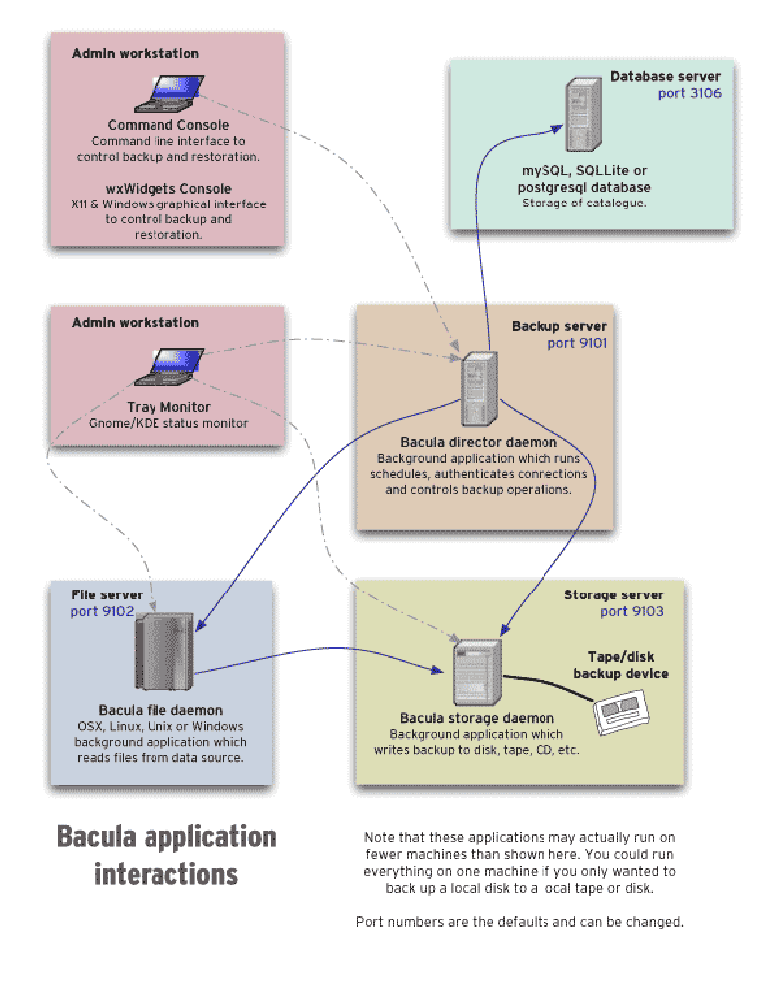
\includegraphics[scale=0.8]{../../doc/figuras/bacula-applications.eps}
 % bacula-applications.png: 1179666x1179666 pixel, 0dpi, infxinf cm, bb=
 \caption[Arquitetura geral do Bacula]{Arquitetura geral do sistema \\ \url{http://www.bacula.org/en/dev-manual/What_is_Bacula.html}}
 \label{fig:arqbacula}
\end{figure}

Durante a implementação do patch \patchshort, concentramos apenas nos componentes bacula-dir e catalog database. Não tivemos a necessidade de interferir nos outros componentes do sistema pois tratavam operações nas quais não nos interessavam no momento.

Para ajudar no entendimento, a figura \ref{fig:comparativo} oferece uma visão geral  antes e depois da implementação do patch. 

Na figura \ref{fig:unico} notamos a utilização de um único banco de dados por binário, ou seja, a escolha de qual banco de dados utilizado é definida durante a compilação do código fonte do Bacula, no qual eram definidos os códigos necessários para construir o driver de acesso nativo via API própria de cada banco de dados. A camada sql\_\*.c utiliza as funções definidas em [banco de dados].c,  onde [banco de dados] pode ser apenas um dentre: mysql, postgresql, sqlite. Desta forma, uma vez compilado, o usuário apenas utilizaria o banco de dados escolhido. 
Um outro ponto é o suporte aos bancos de dados limitados, ou seja, apenas para os SGBDs codificados no Bacula.

Já na figura \ref{fig:dbi} observamos um novo cenário no qual uma camada de abstração (via bibliotema libdbi) e um driver (dbi.c) para fazer a interface entre a camada sql\_\*.c e a libdbi foi implementado. Basicamente para garantir dois pontos: 
\begin{itemize}
\item O primeiro é a independência do banco de dados a ser utilizado pelo Bacula. 
\item O segundo ponto é a possibilidade de utilizar vários tipos de SGBDs para armazenar meta-dados de arquivos.                                                                   \end{itemize}
Um exemplo do segundo ponto abordado é a possibilidade de realizar backups entre bancos de dados ou até mesmo a transferência de um catálogo de um banco de dados para outro completamente distinto em caso de problemas ou manutenções.

\begin{figure*}[h]
 \centerline{
  \subfigure[Único banco de dados por binário]{
  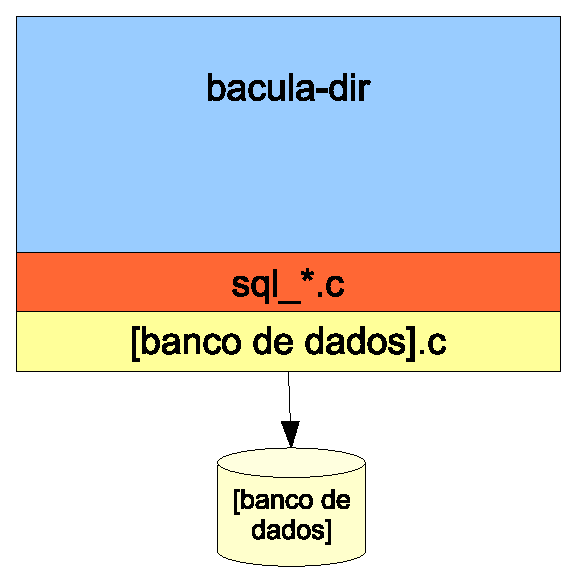
\includegraphics[width=5cm]{../../doc/diagramas/bacula-dir-sgbd.eps}
  \label{fig:unico}
  }
  \hfil
  \subfigure[Vários tipos de banco de dados por binário]{
  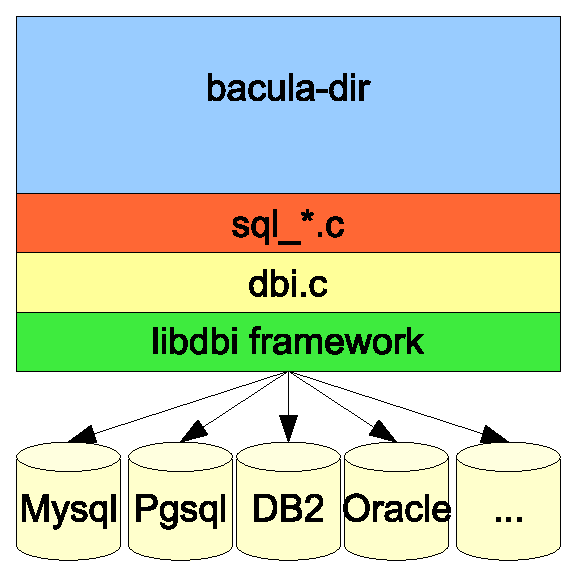
\includegraphics[width=5cm]{../../doc/diagramas/bacula-dir-dbi.eps}
  \label{fig:dbi}
  }
 } 
 \label{fig:comparativo}
 \caption[Comparativo de implementação]{Comparativo da implementação realizada \subref{fig:unico} e \subref{fig:dbi}}
\end{figure*}

\subsection{Limitações}

A principal limitação encontrada é referente a existência de diversos tipos de SGBDs utilizando diferentes dialetos e recursos da linguagem SQL. Não é possível prever todos os casos. Há consultas que funcionam em todos os SGBDs e outras que são específicas e devem ser tratadas a parte. 

A biblioteca libdbi oferece uma abstração para os diferentes tipos de APIs de cada fabricante de SGBDs mas a mesma não oferece nenhum suporte aos diferentes tipos de SQL utilizados por eles.

Sendo assim o Bacula deve ser preparado para suportar os diferentes dialetos SQL, ou seja, para cada banco de dados temos um conjunto de SQL que devem ser adptadas e suportadas para que o SGBD seja efetivamente suportado. Isso se torna uma limitação pois necessita de uma intervenção no código para o correto funcionamento.

\subsection{Implementação}

As tarefas de criação do ambiente necessário para a implementação e definição de quais arquivos seriam necessários criar ou alterar não foram complicadas. Notamos um software bem modularizado e dividido para facilitar a manutenção e adiçaõ de novos recursos. A seguir apresentamos uma macro lista dos itens no qual foram necessário trabalhar:

\begin{itemize}
\item Alteração no arquivo \url{src/cats/cats.h}: 
 \subitem inclusão da regra de compilação condicional HAVE\_DBI para o compilador reconhecer o código para o driver DBI
 \subitem adaptado a estrutura de dados B\_DB, responsável pelo gerenciamento de todos os itentes relacionados a banco de dados, dentro do Bacula, bem como as definições de várias funções para a API da libdbi
\item Alteração dos arquivos \url{src/cats/sql*.c}: incluindo a regra de compilação condicional HAVE\_DBI
\item Criado o arquivo \url{src/cats/dbi.c} baseado no código \url{src/cats/postgresql.c}
 \subitem tranformado e convertigo as funções presentes no arquivo src/cats/dbi.c de um código com APIs referentes ao SGBD postgresql para APIs da  biblioteca DBI. Evidente que muitas funções presentes no SGBD postgresql não seguiam a mesma lógica utilizada na biblioteca DBI. Sendo necessário estudar as documentações e códigos de ambas para entender o funcionamento e decidir se a API da biblioteca DBI atendia ou não a forma na qual o Bacula estava projetado para interagir com um SGBD. 
\item Alterado o arquivo \url{src/dird/dird_conf.h} e \url{src/dird/dird_conf.c}
 \subitem adicionado a opção de configuração dbdriver no qual informava ao Bacula qual driver e banco de dados será utilizado.
\item Alterado os arquivos \url{src/autoconf/config.h.in} e \url{src/autoconf/bacula-macros/db.m4} referentes a geração do script de autoconfiguração para compilação, baseados nas disponibilidades dos requisitos da plataforma.
\item Adaptação de todos os testes de regressão para incluir as opções de configuração para o driver DBI
\end{itemize}

\subsection{Timeline do desenvolvimento}
\begin{table}[htbp]
\begin{tabular}{|l|c|c|c|c|}
\hline
 & \textbf{Data} & \textbf{Submissões} & \textbf{Data Integração} & \textbf{Revision} \\ \hline
\multicolumn{ 1}{|c|}{\textbf{Exploração Arquitetural}} & 2007-12-07 &  &  &  \\ \cline{ 2- 5}
\multicolumn{ 1}{|l|}{} & 2008-01-11 &  &  &  \\ \hline
\multicolumn{ 1}{|c|}{\textbf{Desenvolvimento}} & 2008-01-18 &  &  &  \\ \cline{ 2- 5}
\multicolumn{ 1}{|l|}{} &  & 2008-02-01 & 2008-02-02 & 6358 \\ \cline{ 2- 5}
\multicolumn{ 1}{|l|}{} &  & 2008-02-12 & 2008-02-13 & 6413 \\ \cline{ 2- 5}
\multicolumn{ 1}{|l|}{} &  & 2008-02-19 & 2008-02-22 & 6464 \\ \cline{ 2- 5}
\multicolumn{ 1}{|l|}{} &  & 2008-02-21 & 2008-02-27 & 6498 \\ \cline{ 2- 5}
\multicolumn{ 1}{|l|}{} &  & 2008-02-25 & 2008-04-15 & 6825 \\ \cline{ 2- 5}
\multicolumn{ 1}{|l|}{} &  & 2008-03-17 & 2008-04-15 & 6826 \\ \cline{ 2- 5}
\multicolumn{ 1}{|l|}{} &  & 2008-04-09 & 2008-04-09 & 6817 \\ \cline{ 2- 5}
\multicolumn{ 1}{|l|}{} &  & 2008-04-14 & 2008-04-15 & 6818 \\ \cline{ 2- 5}
\multicolumn{ 1}{|l|}{} &  & 2008-04-27 & 2008-04-27 & 6874 \\ \cline{ 2- 5}
\multicolumn{ 1}{|l|}{} & 2008-05-02 &  &  &  \\ \hline
 &  &  &  &  \\ \hline
 & \textbf{Orçadas} & \textbf{Trabalhadas} &  &  \\ \hline
\textbf{Exploração Arquitetural:} & 64h & 59.89h &  &  \\ \hline
\textbf{Desenvolvimento:} & 168h & 118h &  &  \\ \hline
\end{tabular}
\caption{Timeline}
\label{Timeline}
\end{table}

% \newpage
% Copyright (c) 2008, João Henrique Ferreira de Freitas
% All rights reserved.
% 
% Redistribution and use in source and binary forms, with or without modification,
% are permitted provided that the following conditions are met:
% 
%     * Redistributions of source code must retain the above copyright notice,
%       this list of conditions and the following disclaimer.
%     * Redistributions in binary form must reproduce the above copyright notice,
%       this list of conditions and the following disclaimer in the documentation and/or 
%       other materials provided with the distribution.
%     * Neither the name of the <ORGANIZATION> nor the names of its contributors may
%       be used to endorse or promote products derived from this software without 
%       specific prior written permission.
% 
% THIS SOFTWARE IS PROVIDED BY THE COPYRIGHT HOLDERS AND CONTRIBUTORS "AS IS" AND ANY 
% EXPRESS OR IMPLIED WARRANTIES, INCLUDING, BUT NOT LIMITED TO, THE IMPLIED WARRANTIES
% OF MERCHANTABILITY AND FITNESS FOR A PARTICULAR PURPOSE ARE DISCLAIMED. IN NO EVENT
% SHALL THE COPYRIGHT OWNER OR CONTRIBUTORS BE LIABLE FOR ANY DIRECT, INDIRECT, INCIDENTAL,
% SPECIAL, EXEMPLARY, OR CONSEQUENTIAL DAMAGES (INCLUDING, BUT NOT LIMITED TO, PROCUREMENT
% OF SUBSTITUTE GOODS OR SERVICES; LOSS OF USE, DATA, OR PROFITS; OR BUSINESS INTERRUPTION)
% HOWEVER CAUSED AND ON ANY THEORY OF LIABILITY, WHETHER IN CONTRACT, STRICT LIABILITY,
% OR TORT (INCLUDING NEGLIGENCE OR OTHERWISE) ARISING IN ANY WAY OUT OF THE USE OF THIS
% SOFTWARE, EVEN IF ADVISED OF THE POSSIBILITY OF SUCH DAMAGE.
% 
% $Id$

\section{Anexo F: Sobre o projeto libdbi} \label{sec:anexog}

O projeto libdbi \url{http://libdbi.sourceforge.net} visa a implementação de uma camada de abstração em C para banco de dados. A idéia principal é a utilização de uma camada genérica de código que pode tratar múltiplos acessos a vários bancos de dados simultâneamente. 

A licença utiliza pela libdbi, incluindo os drivers de acesso para os seguintes bancos de dados: Firebird/Interbase, FreeTDS (MS SQL), MySQL, SQLite/SQLite3, Postgresql, Ingres, Oracle, é a LGPL.

Alguns pontos fortes nos quais foram fundamentais para a escolha da libdbi para a experiência foram: 

\begin{description}
 \item[Abstração do banco de dados]: a libdbi manipula todos os detalhes relacionados ao banco de dados. 
 \item[Modularidade]: o usuário pode escolher qual banco de dados deseja apenas alterando uma simples configuração.
 \item[Interface limpa]: possui uma excelente API de fácil entendimento e uma boa documentação da mesma. Facilitando a escrita do software para vários bancos de dados diferentes ao mesmo tempo.
 \item[Driver interface]: possui recursos de carga de drivers para acesso a banco de dados dinâmicamente. Os drivers podem ser facilmente escritos e não necessitam de instalação especial.
 \item[Conveniencia]: não nos preocupamos em escrever o software baseado em recursos de diretivas de compilação (\#define) como geralmente software com acesso a múltiplos bancos de dados fazem.
 \end{description}

\subsection{Interação com o projeto Bacula}

Quando iniciamos o desenvolvimento para adicionar uma camada de abstração para acesso a banco de dados no projeto Bacula, tinhamos a necessidade de encontrar uma biblioteca já pronta para usar, aderente a uma licença não restritiva, madura e estável. Após algumas pesquisas, encontramos a biblioteca libdbi com todos os requisitos desejados.

O primeiro passo foi verificar a estabilidade. Questionando a base de usuários e desenvolvedores, no qual nos esclareceu diversas dúvidas sobre o produto. Em seguida fizemos algumas explorações arquiteturais e testes com a biblioteca com objetivos de aprender os conceitos. A última etapa foi usá-la no desenvolvimento do patch para o Bacula.

Diversas necessidades surgiram durante o desenvolvimento da integração com o Bacula, alguns exemplos abaixo, e foram sanadas ao longo do ciclo de desenvolvimento:

\begin{itemize}
 \item Correções em funções de retorno de erro nas quais em determinadas ocasiões não era possível obter o resultado da última operação executada no banco de dados (Revisão 1.78 \url{libdbi/src/dbi_main.c});
 \item Inicialmente, até a versão 0.8.3 a biblioteca libdbi possuia funções para fazer o escape de querys no banco de dados. Entretanto as funções de escape adicionavam aspas simples no início da string e no final. Este comportamento não era desejado pois o Bacula fazia a inserção de aspas simles nas strings. Após algumas investigações, escrita de patchs para as funções desejadas e discussão com desenvolvedores, foi integrado no repositório CVS as melhorias referentes a não adicionar o símbolo de aspas simples após a string ser \textit{escapada} (Revisão 1.79 \url{libdbi/src/dbi_main.c});
 \item Mudança de conceitos relacionados ao instânciamento de conexões com banco de dados dentro da biblioteca libdbi. Esta mudança ofereceu suporte necessário para utilização de vários bancos de dados ao mesmo tempo. Inicialmente não haviamos detectado problemas com o antigo conceito utilizado pela libdbi. As mudanças foram feitas por outros desenvolvedores externos a libdbi e integradas ao projeto (Revisão 1.81 \url{libdbi/src/dbi_main.c});
 \item Um outro ponto foi o suporte a utilização de funções específicas do banco de dados e não contempladas pela libdbi. Como por exemplo: construções de insert com o comando COPY do Postgresql\footnote{\url{http://www.postgresql.org/docs/8.2/interactive/libpq-copy.html}}. Até a versão 1.0.0 da libdbi não era possível. Após investigações e discussões conseguimos fazer funcionar o suporte a funções específicas dentro da libdbi (Revisão 1.82 \url{libdbi/src/dbi_main.c} e Revisão 1.57 \url{libdbi-drivers/drivers/pgsql/dbd_pgsql.c}), dando suporte ao recursos conhecido, no projeto Bacula, como \textit{batch insert}.
\end{itemize}

Enfim, utilizar a biblioteca libdbi no projeto Bacula poupou várias horas de desenvolvimento, análise de problemas. Além do suporte, desejado, a vários bancos de dados diferentes em uma única implementação.

\end{document}
